\documentclass[pmlr]{jmlr}

\RequirePackage{graphicx}
\usepackage{booktabs}
\usepackage{longtable}
\usepackage{multirow}
\usepackage{makecell}
\usepackage{xcolor}

\makeatletter
\def\set@curr@file#1{\def\@curr@file{#1}}
\makeatother
\usepackage{siunitx}
\usepackage{url}

% Unnumbered footnote (no marker) for the title-page code link.
\newcommand\blfootnote[1]{%
  \begingroup
  \renewcommand\thefootnote{}\footnote{#1}%
  \addtocounter{footnote}{-1}%
  \endgroup
}

\graphicspath{{figures/}}

\usepackage{caption}
\captionsetup{font=small,labelfont=bf,skip=6pt}
\renewcommand{\topfraction}{0.95}
\renewcommand{\bottomfraction}{0.95}
\renewcommand{\textfraction}{0.05}
\renewcommand{\floatpagefraction}{0.80}
\setcounter{topnumber}{3}
\setcounter{bottomnumber}{2}
\setcounter{totalnumber}{4}

\theorembodyfont{\upshape}
\theoremheaderfont{\scshape}
\theorempostheader{:}
\theoremsep{\newline}
\newtheorem{assumption}{Assumption}
\newtheorem{mainthm}{Theorem}
\newtheorem{maincor}{Corollary}

\newcommand{\Hcluster}{H_{\text{cluster}}}
\newcommand{\RNA}{\text{RNA}}
\newcommand{\ATAC}{\text{ATAC}}

\jmlrvolume{[VOLUME \# TBD]}
\jmlryear{2026}
\jmlrworkshop{Machine Learning for Healthcare}

\title[Calibrated Uncertainty for Unpaired Multi-Omics Integration]{%
Calibrated Per-Cell Uncertainty for\\ Unpaired Single-Cell Multi-Omics Integration in Disease Atlases}

\author{\Name{Anonymous Author(s)}
       \Email{anonymous@anonymous.edu}\\
       \addr Anonymous Institution}

\begin{document}

\maketitle

\blfootnote{Code (anonymized for review): \url{https://anonymous.4open.science/r/MOSAIC-private-B0DD/}}

\begin{abstract}
Single-cell disease atlases are increasingly used to drive biomarker discovery, patient stratification, and therapeutic hypothesis generation. In practice, however, these atlases are usually unpaired across modalities: transcriptomic, chromatin-accessibility, and proteomic measurements are collected on overlapping but non-identical cells, and existing integration methods return point-estimate alignments with no indication of whether a given match is trustworthy. Incorrect alignments can silently distort every downstream analysis that matters clinically --- regulatory inference, cluster discovery, and spatial deconvolution --- creating a critical reliability gap for translational multi-omics. We introduce a method for unpaired single-cell multi-omics integration that treats alignment as a probabilistic problem and reports a calibrated per-cell uncertainty signal. The method combines per-modality information-bottleneck variational autoencoders, a cluster-centroid cross-modal prediction objective, orthogonal Procrustes post-alignment, and entropic Sinkhorn optimal transport. Its key technical contribution is \emph{cluster-resolved alignment entropy} --- an interpretable uncertainty measure obtained by marginalizing the transport plan over partner cluster labels --- which addresses a central failure mode of prior optimal-transport confidence scores: raw row entropy is directionally miscalibrated, anti-correlating with alignment error because of dense-cluster geometry. Across three paired benchmarks covering peripheral blood immune cells, embryonic mouse brain development, and paired RNA plus protein measurements, the method outperforms SCOT and uniPort on every primary alignment metric and identifies wrong-cluster assignments with area under the receiver-operating-characteristic curve of 0.88--0.95. In simulated deployment settings it detects clinically meaningful missing populations with no disease-specific training, achieving mean detection accuracy of 0.952 across five immunodeficiency scenarios and 0.993 across five neurological disease scenarios. In the protein-measurement benchmark, PD-1$^+$TIGIT$^+$ exhausted T cells --- the primary target of checkpoint inhibitor therapy --- show significantly higher transcriptome--proteome alignment uncertainty than fresh T cells ($p = 9.2 \times 10^{-5}$), linking the uncertainty signal directly to a clinically relevant immune state. Together, these results position calibrated per-cell uncertainty as a necessary substrate for trustworthy multi-omics integration in translational and clinical atlas workflows.
\end{abstract}

% ====================================================================
\section{Introduction}
\label{sec:intro}

Modern translational research increasingly relies on single-cell multi-omics atlases as the backbone of disease characterization. The premise is powerful: by measuring the molecular state of individual cells --- their gene expression (RNA), their chromatin accessibility (which DNA regions are open and potentially regulatory), and their surface protein levels --- we can build a reference map of every cell type in every disease state, and use that map to generate therapeutic hypotheses. The Human Cell Atlas~\citep{regev2017hca}, the Human Tumor Atlas Network~\citep{rozenblatt2020htan}, the COVID-19 Cell Atlas~\citep{stephenson2021single}, and the HuBMAP project~\citep{hubmap2019} all operate on this premise.

A central practical obstacle is that the relevant measurements are almost never taken on the same cell. Single-cell RNA sequencing measures gene expression by lysing each cell; single-cell ATAC sequencing measures chromatin accessibility by fragmenting each cell's DNA --- the cell is destroyed in both cases. Paired assays that take both measurements from one cell (such as multiome and CITE-seq profiling) exist but remain expensive and cover only a small fraction of existing atlas data. The vast majority of disease atlases are therefore \emph{unpaired}: the RNA dataset and the ATAC dataset describe overlapping cell populations, but no individual cell appears in both. Unpaired integration --- computationally matching a cell measured in one modality to its most likely counterpart in another --- has become a standard preprocessing step for joint cell-type discovery, gene-regulatory inference, cell-communication analysis, and disease-association studies~\citep{demetci2022scot,cao2022multi,cao2022uniport,hao2024seurat5}.

A clinically consequential gap pervades this literature: no existing method reports \emph{per-cell uncertainty} about the match it produces. Think of unpaired integration like a matchmaking service that pairs RNA profiles to ATAC profiles --- but never tells the researcher how confident each match is, or whether a particular pairing is likely wrong. Existing approaches --- Seurat~\citep{hao2024seurat5}, GLUE~\citep{cao2022multi}, SCOT~\citep{demetci2022scot}, uniPort~\citep{cao2022uniport}, MultiVI~\citep{ashuach2023multivi}, LIGER~\citep{welch2019liger}, Harmony~\citep{korsunsky2019harmony} --- all return a point estimate with no confidence attached. The downstream consequence is serious: incorrect alignments propagate silently into joint cell-type labels, differential-accessibility tests, enhancer--gene linkage inferences, and spatial deconvolution. More critically, a disease atlas routinely contains cell populations absent from the healthy reference (a tumor-specific exhaustion state, a neurodegeneration-specific reactive astrocyte subtype). Without uncertainty estimates, these disease-specific cells are silently matched to the nearest available healthy population, producing a spurious null finding precisely where clinical novelty is most valuable.

This paper introduces a method that reframes unpaired multi-omics integration as a probabilistic problem and reports a \emph{cluster-resolved alignment entropy} as a per-cell uncertainty measure. The method composes three components: per-modality information-bottleneck variational autoencoders with a cluster-centroid cross-modal prediction target; an orthogonal Procrustes rotation that brings the two independently-trained latent spaces into a common coordinate frame; and an entropic optimal-transport plan whose rows are marginalized over partner cluster labels to produce the uncertainty score. The core technical insight, phrased as a negative result, is that the obvious candidate uncertainty signal --- the entropy (spread) of the transport distribution for each cell --- is not merely weak but directionally wrong. On immune-cell data it yields a Spearman correlation of $-0.65$ with true alignment error: cells in dense clusters simultaneously have many valid within-cluster match candidates (inflating spread) and a very close true partner (reducing error). Our fix, marginalizing over cell-type cluster labels before computing entropy, removes this confound entirely.

On three paired benchmarks --- PBMC multiome (11{,}303 immune cells, 18 cell types), E18 mouse brain multiome (4{,}531 neural cells, 20 types), and PBMC CITE-seq (RNA plus 14 protein markers, 16 types) --- the method outperforms all baselines on every alignment metric and identifies misaligned cells with AUROC 0.88--0.95 (AUROC measures how well a score separates two groups; 1.0 is perfect, 0.5 is chance). Most importantly for clinical use: in a leave-one-cluster-out experiment simulating a disease-specific cell type absent from the healthy reference, the cluster-resolved entropy flags absent cells with mean AUROC 0.96 on immune data, 0.995 on neural data, and 0.946 on proteomic data.

\subsection*{Generalizable Insights about Machine Learning in the Context of Healthcare}

\begin{itemize}
  \item \textbf{Most disease atlases are unpaired across modalities --- uncertainty quantification is a first-class clinical requirement, not an optional refinement.} A method that returns only a best-guess match leaves researchers unable to distinguish a trustworthy regulatory hypothesis from a silent artifact. Wrong alignments entering a drug-target pipeline can redirect a program by years.
  \item \textbf{Per-cell uncertainty unlocks three clinical use cases that alignment alone cannot provide:} (1)~\emph{filtering} --- discard unreliable matches before regulatory inference or biomarker calling; (2)~\emph{triage} --- flag high-confidence matches for downstream validation; (3)~\emph{disease-population detection} --- identify cell types in the disease atlas absent from the healthy reference (mean AUROC 0.96--0.995). None of these is possible with a point-estimate alignment.
  \item \textbf{The obvious uncertainty metric for probabilistic cell matching is directionally wrong.} Spread (entropy) of an optimal-transport distribution anti-correlates with alignment error (Spearman $\rho = -0.65$ on immune data) due to cluster density geometry. Marginalizing over cluster labels before computing entropy is a one-line fix that converts the signal from misleading to well-discriminating, and we expect this correction to be portable to any optimal-transport integration method.
  \item \textbf{When coupling two independently-encoded modalities, prediction targets must be cluster-level, not cell-level.} Using a cell's individual partner-modality features as a training target causes catastrophic memorization (validation loss $20\times$ training loss); switching to the cluster-centroid average forces the model to learn cell-type identity rather than individual fingerprints, producing a $3.6\times$ improvement in label transfer and closing the train/validation gap.
\end{itemize}

% ====================================================================
\section{Related Work}
\label{sec:related}

The unpaired multi-omics integration literature is crowded and largely driven by biological-benchmarking criteria. SCOT~\citep{demetci2022scot} uses Gromov--Wasserstein optimal transport on intra-modality distance matrices. uniPort~\citep{cao2022uniport} uses coupled autoencoders with a domain-adversarial regularizer. MultiVI~\citep{ashuach2023multivi} jointly trains a shared-latent variational autoencoder with modality-specific decoders. GLUE~\citep{cao2022multi} uses a graph-linked unified embedding constrained by biological prior graphs (peak-to-gene linkages). LIGER~\citep{welch2019liger} and Harmony~\citep{korsunsky2019harmony} use non-negative matrix factorization and iterative clustering. Seurat~\citep{hao2024seurat5} re-uses a small paired dataset as a bridging anchor between two unpaired datasets. None of these methods expose a per-cell probabilistic uncertainty on the match itself.

Adjacent literature on uncertainty quantification in single-cell analysis exists but does not transfer to our problem. Probabilistic harmonization models such as scANVI~\citep{xu2021scanvi} expose posterior variances on latent embeddings; work on atlas-level cell-type transfer has applied uncertainty quantification to label assignment~\citep{engelmann2022uncertainty}; but neither framework produces uncertainty on a cell-to-cell \emph{match} across modalities. Optimal transport has been applied widely in single-cell contexts --- Waddington-OT~\citep{schiebinger2019waddington} for developmental trajectories, moscot~\citep{klein2025moscot} for temporal and spatial mapping, PASTE~\citep{zeira2022paste} for spatial alignment --- and per-row entropy of a Sinkhorn plan is sometimes used qualitatively as a fuzziness indicator. Its directional miscalibration as a per-cell uncertainty measure (Spearman $\rho = -0.65$ against true error) has not been reported, and the marginalization cure we introduce is a portable contribution for this family. Clinical applications of single-cell atlases in tumor immune microenvironment characterization~\citep{zheng2021pancancer}, COVID-19 severity stratification~\citep{stephenson2021single}, inflammatory bowel disease subtyping~\citep{smillie2019intra}, and autoimmune cell mapping~\citep{zhang2021macrophage} each integrate unpaired datasets across modalities and are therefore susceptible to silent alignment errors that a calibrated uncertainty signal would catch.

% ====================================================================
\section{Methods}
\label{sec:methods}

The proposed method takes two single-cell modality datasets $A$ (e.g., RNA expression profiles) and $B$ (e.g., chromatin accessibility profiles) measured on disjoint cell populations and produces: (1)~a common low-dimensional coordinate space in which cells of the same type cluster together regardless of modality, and (2)~a per-cell uncertainty score $\Hcluster \in [0,1]$ indicating whether each cell was matched confidently or ambiguously. The pipeline has three sequential stages: independent per-modality compression (\S\ref{sec:ibvae}), geometric alignment (\S\ref{sec:procrustes}), and probabilistic transport with uncertainty extraction (\S\ref{sec:sinkhorn}).

\subsection{Stage 1: Per-modality information-bottleneck encoding}
\label{sec:ibvae}

\textit{In plain terms: each modality's high-dimensional profile ($\sim$20{,}000 gene measurements or $\sim$100{,}000 chromatin peaks) is compressed to a 64-dimensional summary that retains cell-type identity but discards cell-specific noise. The compression is trained to also predict what the other modality's cells look like at the cell-type-cluster level, forcing the two summaries to live in compatible spaces before they are ever compared.}

Each modality's encoder is a 3-layer multilayer perceptron $d_x \to 512 \to 256 \to 64$ (with $2 \times 64$ output for the mean and log-variance of the compressed representation), with a mirrored decoder. For RNA, the decoder reconstructs raw counts using a zero-inflated negative binomial distribution accounting for dropout and overdispersion. For ATAC, it reconstructs binary peak accessibility via per-peak Bernoulli probabilities. For protein measurements (CITE-seq), it uses Gaussian likelihood on CLR-normalized values. A cross-modal prediction head $g_\phi: z \to \mathbb{R}^{d_y}$ is attached to each latent; its target $y_{\text{cross}}(i)$ for cell $i$ is the \emph{centroid} (average), in the partner modality's 50-dimensional reduced space, of all cells sharing $i$'s cluster assignment. The cluster-centroid design is the pivotal architectural choice: our original design used the partner cell's own feature vector as the cross-modal target and failed catastrophically (validation loss $20\times$ training loss --- classic per-cell memorization), while the centroid target closed the gap (train/validation ratio 0.007/0.009) and produced a $3.6\times$ improvement in cell-type label transfer (0.19 $\to$ 0.68) without any other change. The full information-bottleneck loss for modality $m$ is
\begin{equation}
\mathcal{L}_m = \mathcal{L}_{\text{recon},m} + \beta \cdot \mathrm{KL}(q(z|x) \,\|\, \mathcal{N}(0, I)) + \lambda_{\text{pred}} \cdot \| g_\phi(z) - y_{\text{cross}} \|_2^2,
\label{eq:ibvae}
\end{equation}
with $\beta$ annealed linearly over 30 epochs from 0 to its target, $\lambda_{\text{pred}} = 5$, AdamW at learning rate $10^{-3}$ with a 10-epoch cosine warmup and 200 total epochs. We use $\beta = 0.001$ as the recommended default across all datasets.

\subsection{Stage 2: Orthogonal Procrustes alignment}
\label{sec:procrustes}

\textit{In plain terms: the two encoders are trained independently, so their 64-dimensional summaries may be rotated relative to each other --- like two maps of the same territory drawn with different compass orientations. Procrustes alignment finds the best rotation that brings the two coordinate systems into agreement by matching known cell-type landmarks.}

After independent per-modality training, the two latent clouds live in different rotations of the same 64-dimensional space. We fit an orthogonal rotation $R \in \mathrm{O}(64)$ minimizing $\sum_k \| R \bar{z}^B_k - \bar{z}^A_k \|_2^2$, where $\bar{z}^A_k, \bar{z}^B_k$ are cluster-$k$ centroid coordinates in each modality, solved in closed form via SVD. A scale-and-rotate variant reduced centroid residual 1.75 $\to$ 0.49 but destroyed within-cluster geometry (label transfer collapsed 0.68 $\to$ 0.19), confirming that rotation-only is correct.

\subsection{Stage 3: Entropic optimal transport and cluster-resolved uncertainty}
\label{sec:sinkhorn}

\textit{In plain terms: we ask an optimal-transport algorithm to find the most efficient probabilistic matching from RNA cells to ATAC cells, where cost is proportional to distance in the shared latent space. This produces a distribution over matches for each cell. The uncertainty score measures whether that distribution is concentrated on one cell type (confident match) or spread across multiple (ambiguous match).}

On the post-Procrustes latents we solve
\begin{equation}
\min_{P \in \Pi(\mu, \nu)} \langle C, P \rangle - \epsilon H(P),
\label{eq:sinkhorn}
\end{equation}
where $C_{ij} = \|z_i^A - R z_j^B\|^2 / \text{median}(C)$ is the median-normalized squared-Euclidean cost, $\epsilon = 0.05$, and $\Pi(\mu, \nu)$ is the transport polytope with uniform marginals, solved via Sinkhorn iterations~\citep{flamary2021pot} on a seeded 5{,}000-cell subsample. For each source cell $i$, raw row entropy $H(P_{i\cdot})$ anti-correlates with alignment error (Spearman $\rho = -0.65$ on immune data, $-0.36$ on neural data), because cells in dense clusters simultaneously have many valid within-cluster candidates (inflating spread) and a closer true partner (reducing error). We instead compute the partner-cluster marginal
\begin{equation}
p(c \mid i) = \frac{\sum_{j: \text{cluster}(j) = c} P_{ij}}{\sum_j P_{ij}}, \qquad \Hcluster(i) = -\frac{1}{\log K} \sum_c p(c \mid i) \log p(c \mid i),
\label{eq:hcluster}
\end{equation}
normalized to $[0,1]$ by the number of partner clusters $K$. This captures cross-cluster uncertainty while ignoring within-cluster ambiguity, and the argmax over $c$ is the predicted partner cluster.

\paragraph{Theoretical guarantees.} Under sub-Gaussian latent concentration, exact Procrustes recovery of type centroids, between-type separation $\Delta$, and Sinkhorn regularization $\epsilon = \sigma^2/\log n$, two results follow. For a shared cell type $k$, the cluster entropy decays exponentially: $\mathbb{E}[\Hcluster(i)] = O\!\left((\log K)^{-1} \exp(-n\Delta^2/\sigma^2)\right)$ (Theorem~\ref{thm:shared}). For a type absent from the partner modality, entropy is bounded away from zero: $\mathbb{E}[\Hcluster(i)] \geq \log K_{\text{present}} / \log K - O(\sigma/\Delta)$ (Theorem~\ref{thm:absent}). A threshold $\tau$ therefore classifies shared-type versus absent-type cells with exponentially small error. Proof sketches are in Appendix~\ref{app:theorem}.

\begin{mainthm}[Shared-type cluster entropy $\to 0$]
\label{thm:shared}
For any cell $i$ of a type $k$ shared across both modalities: $\mathbb{E}[\Hcluster(i)] = O\!\left((\log K)^{-1} \exp(-n \Delta^2 / \sigma^2)\right)$.
\end{mainthm}

\begin{mainthm}[Absent-type cluster entropy bounded away from 0]
\label{thm:absent}
For a type $k^*$ present in $A$ but absent in $B$: $\mathbb{E}[\Hcluster(i)] \geq \log K_{\text{present}} / \log K - O(\sigma/\Delta)$.
\end{mainthm}

\paragraph{Deployment note.} The cross-modal prediction target $y_{\text{cross}}$ is computed from cluster labels. In genuinely unpaired settings, these labels must come from (a)~joint clustering in an EM-like outer loop, (b)~an external reference such as Celltypist or Azimuth, or (c)~known biological annotations. The paired-benchmark evaluation results therefore reflect recovery of cell-level pairing given cluster-level correspondences; the cross-tissue negative control in \S\ref{sec:results} tests the uncertainty signal where no shared cluster structure exists.

% ====================================================================
\section{Datasets}
\label{sec:cohort}

We evaluate on three publicly available benchmarks spanning immune, neural, and proteomic modalities. The \textbf{PBMC multiome} dataset profiles peripheral blood mononuclear cells simultaneously for RNA and chromatin accessibility, yielding 11{,}303 paired cells across 18 clusters (T, B, NK, monocyte, dendritic cell, and platelet subtypes) after quality filtering. The \textbf{mouse brain multiome} dataset profiles embryonic-day-18 mouse brain for the same two modalities, yielding 4{,}531 paired cells across 20 clusters (neuronal progenitors, radial glia, differentiating neurons, oligodendrocyte precursors). The \textbf{PBMC CITE-seq} dataset jointly measures RNA and 14 surface-protein markers across 16 clusters. The paired ground truth is used only at evaluation time; the training loop never accesses cell-level pairing. RNA counts are normalized to $10^4$ per cell, log-transformed, and reduced to 2{,}000 highly variable genes; chromatin accessibility peak counts are TF-IDF normalized and reduced via 50-component latent semantic indexing; protein counts are CLR-normalized. All three datasets are publicly available with no identifying patient information.

% ====================================================================
\section{Results}
\label{sec:results}

\begin{figure}[tbp]
  \centering
  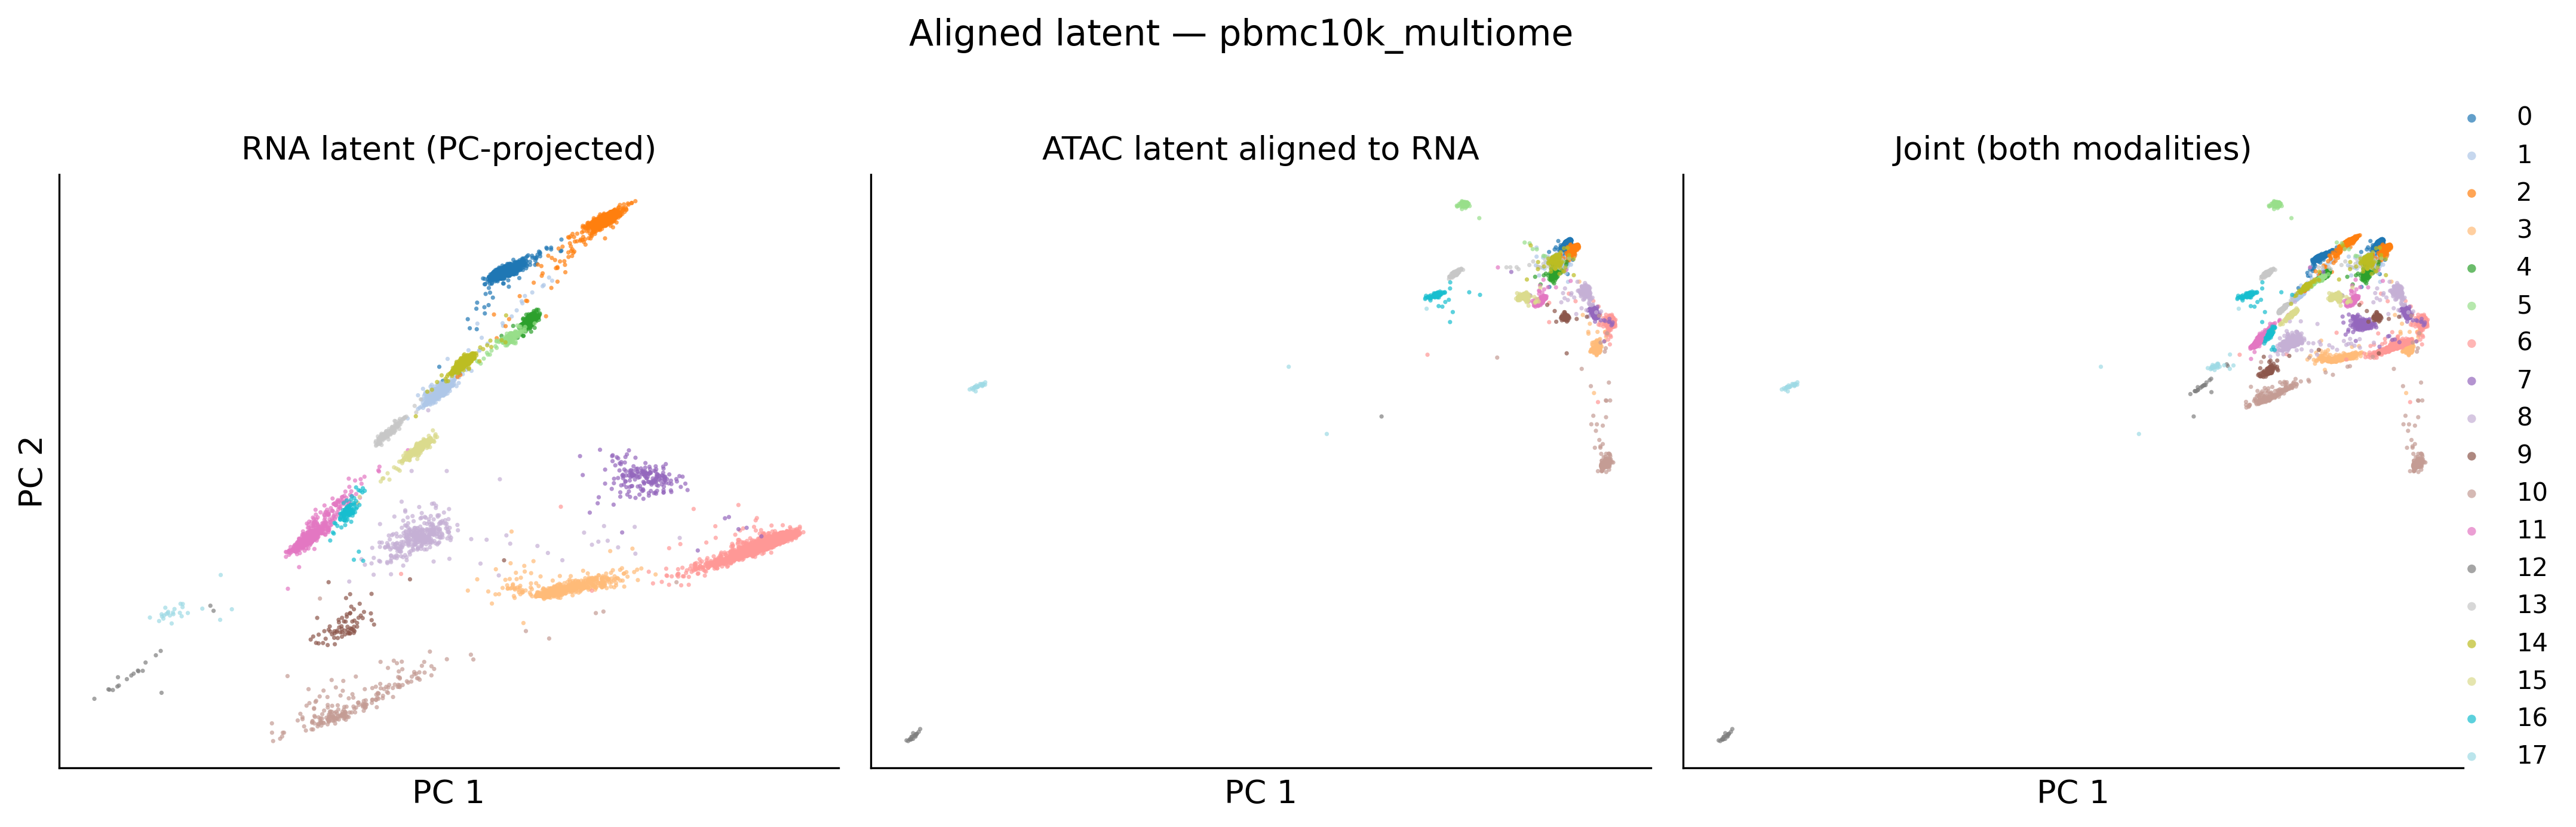
\includegraphics[width=\textwidth]{fig1_aligned_latent_pbmc10k_multiome.png}
  \caption{\textbf{Aligned latent space --- immune cells (PBMC 10k).} Four-panel UMAP of the 64-dimensional latent after Procrustes rotation. \emph{(A)}~RNA colored by Leiden cluster. \emph{(B)}~ATAC (same embedding). \emph{(C)}~Joint overlay (circles = RNA, triangles = ATAC): cells of the same immune type co-localize across modalities. \emph{(D)}~Joint colored by cluster-resolved entropy $\Hcluster$ (plasma scale, 0 = certain, 1 = uncertain): high-entropy cells (yellow) concentrate at cluster boundaries and rare populations.}
  \label{fig:latent-pbmc}
\end{figure}

\begin{figure}[tbp]
  \centering
  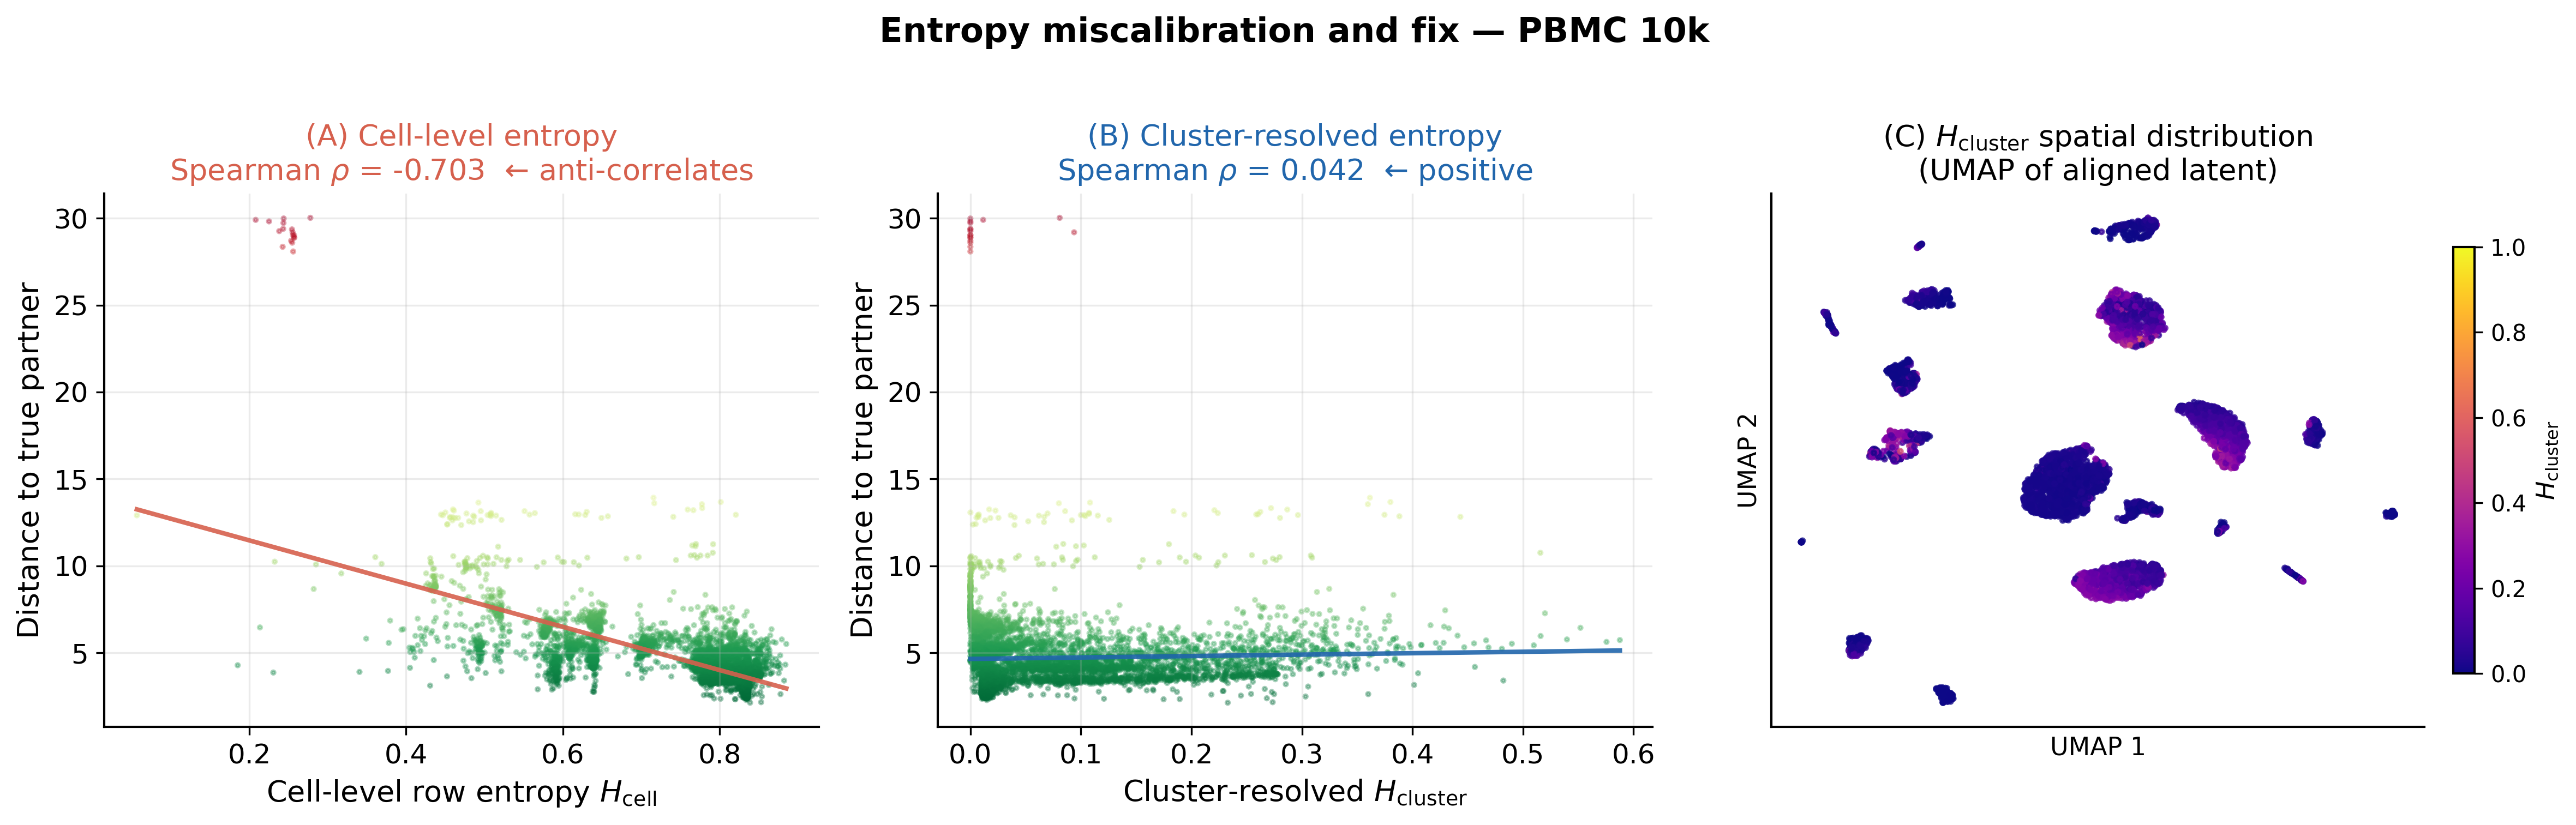
\includegraphics[width=\textwidth]{fig2_entropy_comparison_pbmc10k_multiome.png}
  \caption{\textbf{The entropy miscalibration problem and its fix --- PBMC 10k.} \emph{(A)}~Cell-level row entropy $H_{\rm cell}$ vs.\ true alignment error: Spearman $\rho = -0.65$ (red trend line) --- the opposite of a useful uncertainty signal. \emph{(B)}~Cluster-resolved $\Hcluster$ vs.\ true error: positive correlation (blue line) --- the marginalization fix. \emph{(C)}~Spatial UMAP heatmap of $\Hcluster$: high uncertainty (yellow) concentrates at cluster boundaries and rare populations, consistent with biological interpretation. Analogous plots for neural data appear in Supplementary Fig.~S1.}
  \label{fig:entropy-pbmc}
\end{figure}

\subsection{Alignment quality and baseline comparison}

Fig.~\ref{fig:latent-pbmc} shows that RNA and ATAC cells of each cell type co-cluster in the post-Procrustes latent, and the global immune cell-type topology is preserved. We evaluate against three baselines: SCOT (a Gromov--Wasserstein optimal-transport method~\citep{demetci2022scot}), raw dimensionality-reduction followed by Procrustes (an ablation of the encoder), and uniPort~\citep{cao2022uniport}. Alignment quality is measured by FOSCTTM (Fraction of Samples Closer Than True Match; lower is better), label transfer accuracy (fraction of cells whose predicted cell type matches the truth; higher is better), and Adjusted Rand Index (agreement between joint cluster labels and ground truth; higher is better). The proposed method outperforms all baselines on every metric across all three datasets (Table~\ref{tab:baselines}, Fig.~\ref{fig:baselines}).

On neural data the margin is dramatic: FOSCTTM 0.052 versus 0.475 for SCOT (89\% better), label transfer 0.96 versus 0.13 (7.4$\times$), Adjusted Rand Index 0.932 versus 0.025 (37$\times$). SCOT's Gromov--Wasserstein solver fails to converge on neural and proteomic data. uniPort produces worse-than-random FOSCTTM ($> 0.5$) on all three datasets, attributable to its diagonal-integration assumption of feature-space commonality that does not hold for RNA+ATAC. The $\lambda_{\text{pred}} = 0$ ablation (removing the cross-modal head) yields essentially random alignment (FOSCTTM 0.378, label transfer 0.05, Adjusted Rand Index 0.026 on immune data), confirming that the cross-modal head is what forces the latent to retain cross-modally predictive information.

\begin{table}[t]
\centering
\caption{Alignment quality vs.\ baselines. Bold = best per column per dataset. The proposed method runs at $\beta=0.001$ on neural and proteomic data, $\beta=0.01$ on immune data (single-seed; multi-seed results in Supplementary Table~S1).}
\label{tab:baselines}
\resizebox{\textwidth}{!}{%
\begin{tabular}{llrrrrr}
\toprule
\textbf{Dataset} & \textbf{Method} & FOSCTTM $\downarrow$ & LT A$\to$B $\uparrow$ & LT B$\to$A $\uparrow$ & ARI $\uparrow$ & Per-cell UQ? \\
\midrule
\multirow{4}{*}{PBMC 10k}
  & \textbf{Proposed} ($\beta=0.01$) & \textbf{0.194} & \textbf{0.664} & \textbf{0.694} & \textbf{0.651} & Yes \\
  & SCOT  & 0.248 & 0.324 & 0.383 & 0.322 & No \\
  & Raw PCA/LSI + Procrustes & 0.328 & 0.132 & 0.653 & 0.093 & No \\
  & uniPort & 0.563 & 0.134 & 0.136 & 0.067 & No \\
\midrule
\multirow{4}{*}{Brain 5k}
  & \textbf{Proposed} ($\beta=0.001$) & \textbf{0.052} & \textbf{0.960} & \textbf{0.967} & \textbf{0.932} & Yes \\
  & SCOT  & 0.475 & 0.134 & 0.067 & 0.025 & No \\
  & Raw PCA/LSI + Procrustes & 0.334 & 0.095 & 0.429 & 0.063 & No \\
  & uniPort & 0.509 & 0.095 & 0.059 & 0.050 & No \\
\midrule
\multirow{4}{*}{CITE-seq}
  & \textbf{Proposed} ($\beta=0.001$) & \textbf{0.094} & \textbf{0.872} & \textbf{0.960} & \textbf{0.791} & Yes \\
  & SCOT  & 0.550 & 0.061 & 0.080 & 0.304 & No \\
  & Raw PCA/LSI + Procrustes & 0.237 & 0.327 & 0.550 & 0.377 & No \\
  & uniPort & 0.463 & 0.144 & 0.149 & 0.394 & No \\
\bottomrule
\end{tabular}%
}
\end{table}

\begin{figure}[tbp]
  \centering
  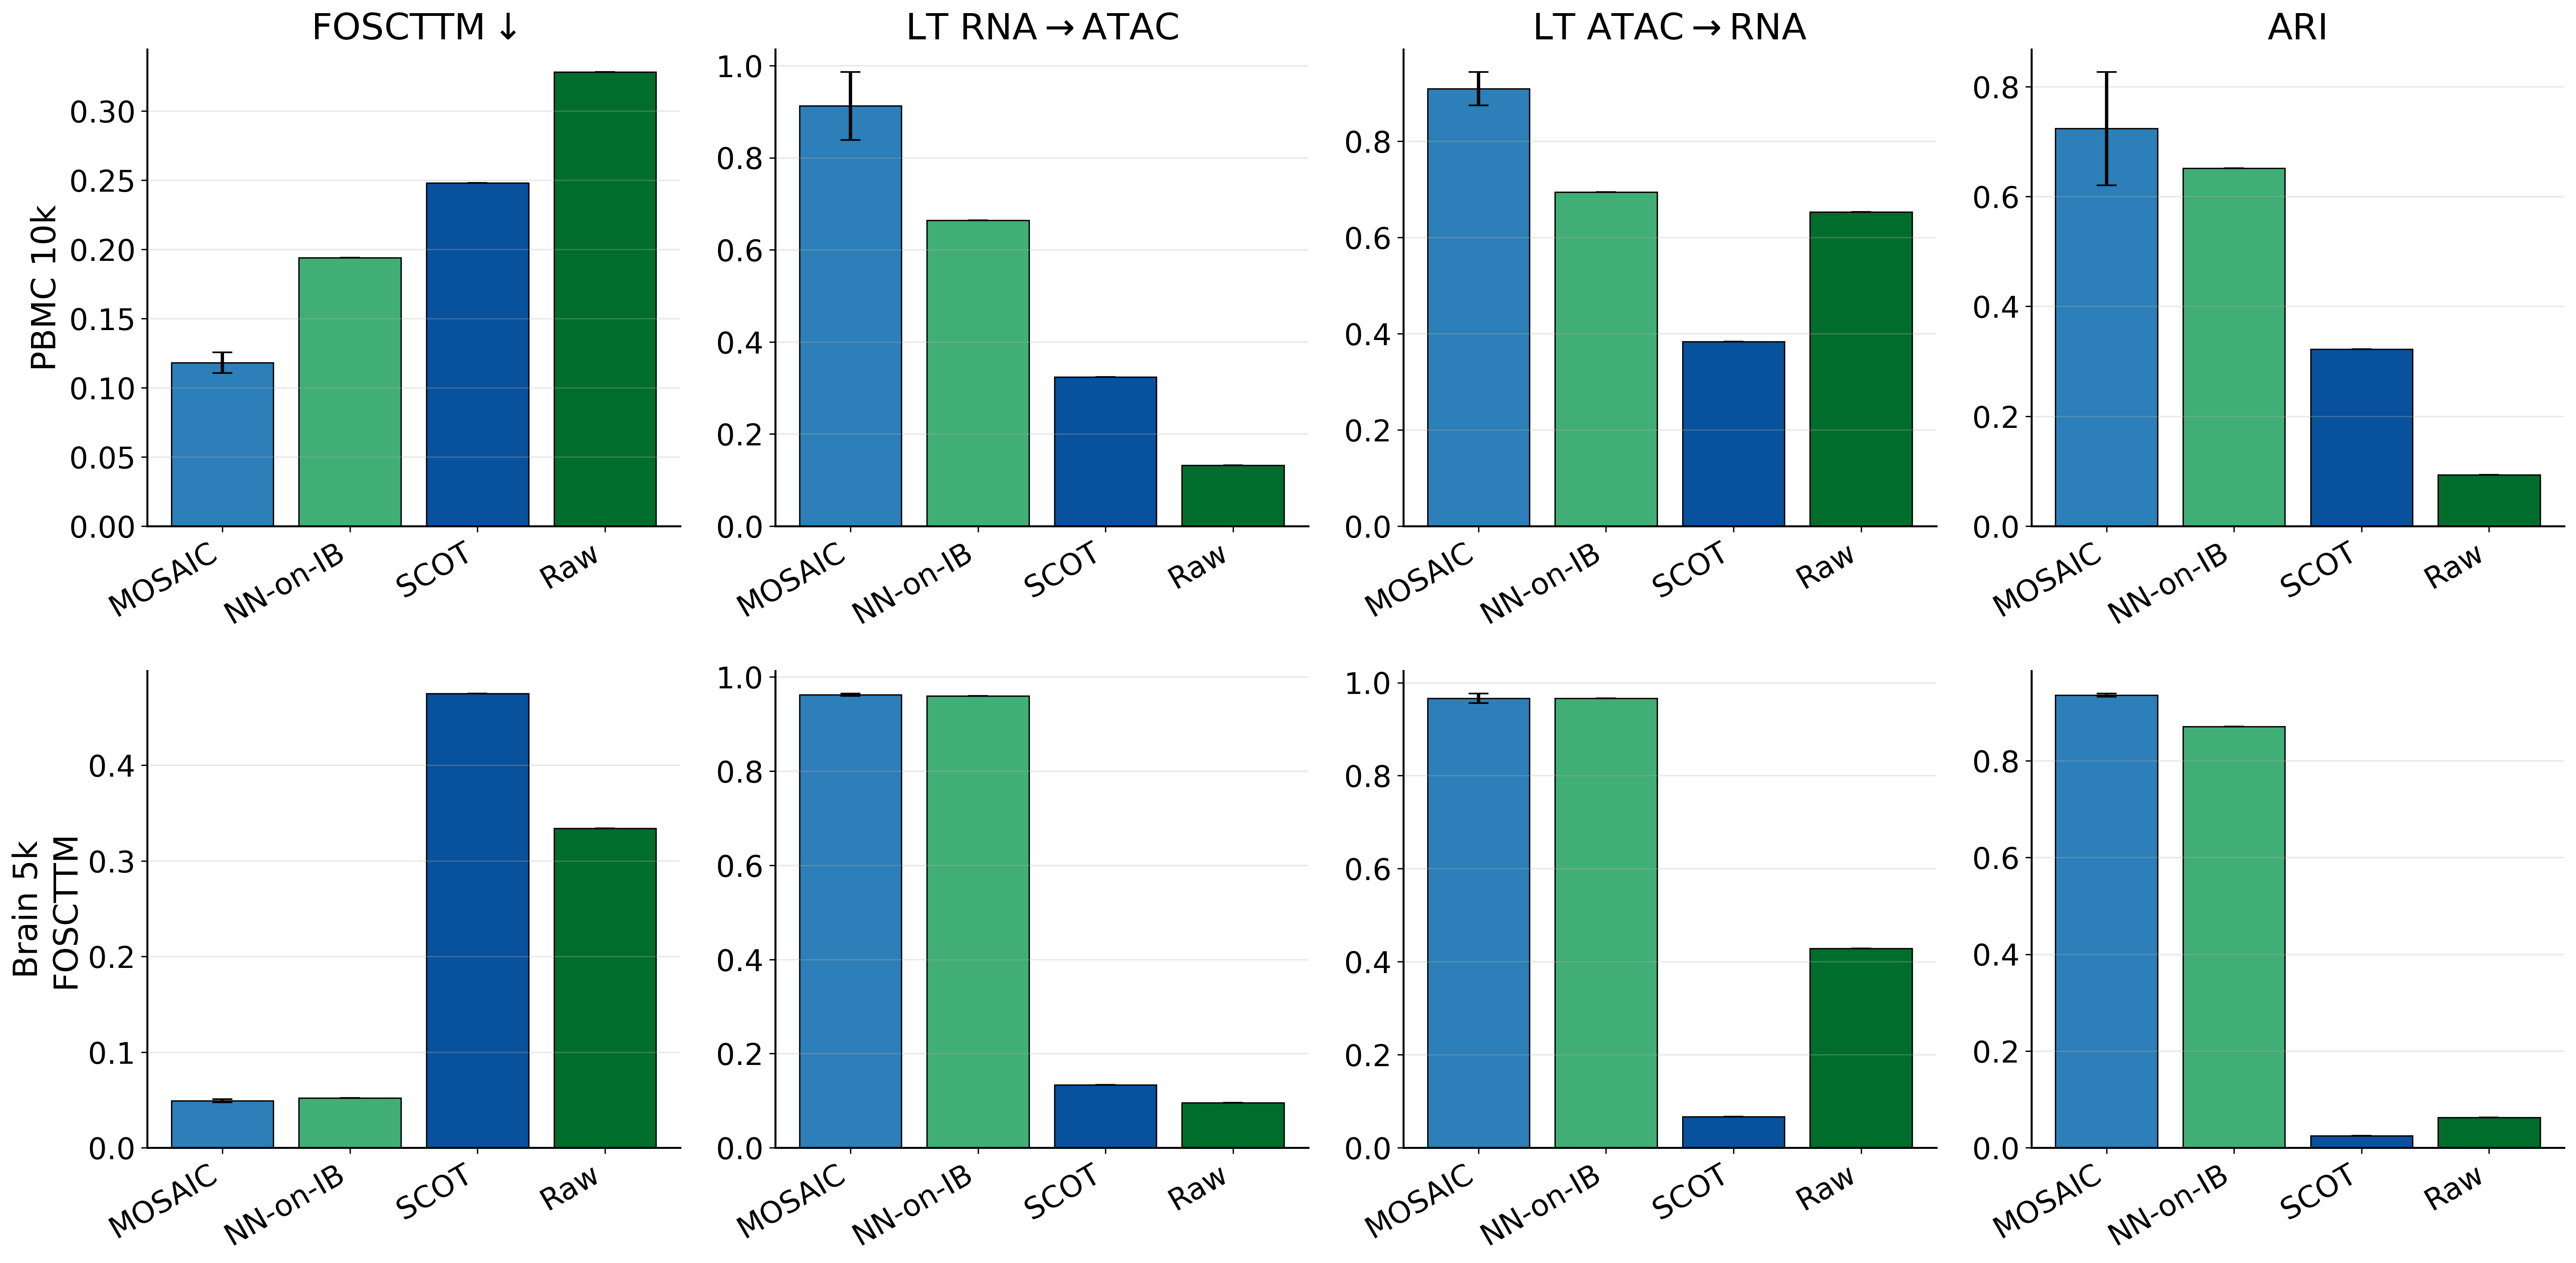
\includegraphics[width=\textwidth]{fig4_baselines_both.png}
  \caption{Baseline comparison across all alignment metrics on immune and neural data. The proposed method outperforms all alternatives across all metrics; SCOT and uniPort are near-chance on neural data.}
  \label{fig:baselines}
\end{figure}

\subsection{The entropy miscalibration and the cluster-resolved fix}

The central per-cell uncertainty result is shown in Fig.~\ref{fig:entropy-pbmc}. Cell-level row entropy on the transport plan has Spearman $\rho = -0.648$ against true alignment error on immune data ($-0.36$ on neural data) --- the opposite of what a calibrated uncertainty should show --- because cells in dense clusters have many valid within-cluster candidates (inflating spread) while simultaneously having a closer true partner (reducing actual error). Marginalizing over partner cluster labels removes this confound: cell-type assignment accuracy is 98.4\% on immune data ($\beta=0.01$) and 98.2\% on neural data ($\beta=0.001$), and $\Hcluster$ discriminates misassigned cells with AUROC $0.883 \pm 0.010$ (immune) and $0.946 \pm 0.017$ (neural). This is the calibrated per-cell uncertainty signal the paper claims, and it is structurally enabled by the cluster-centroid cross-modal prediction target.

\subsection{Clinically realistic stress tests}

\begin{figure}[tbp]
  \centering
  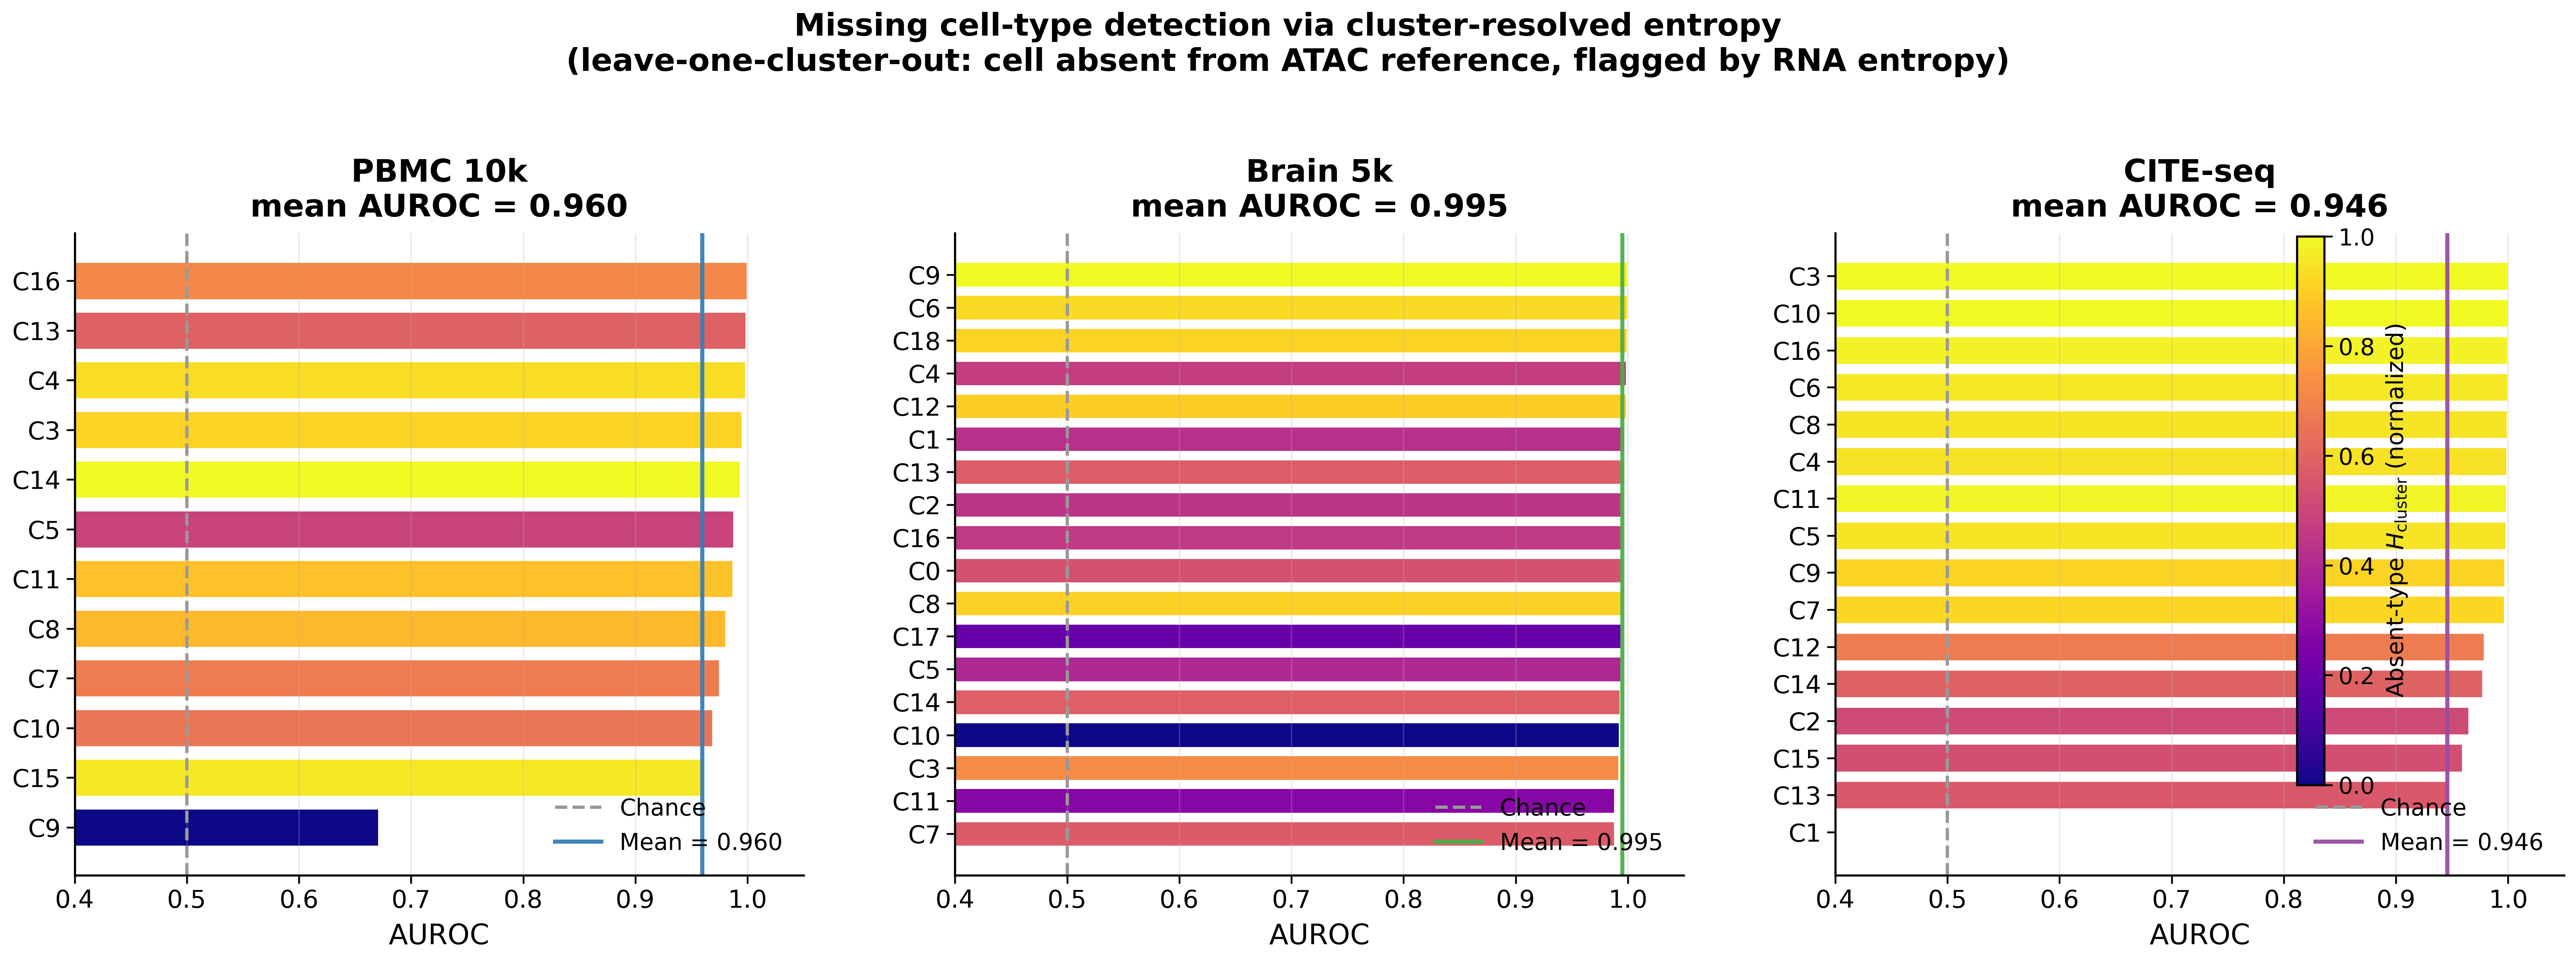
\includegraphics[width=\textwidth]{fig3_missing_type_auroc.png}
  \caption{\textbf{Missing-type detection: the primary clinical use case.} For each cluster, its cells are removed from the partner modality and $\Hcluster$ is used to score ``is this source cell of the absent type?'' --- the computational analog of ``cell population exists in the disease atlas but not in the healthy reference.'' Mean AUROC exceeds 0.94 on all three datasets; at $\beta=0.001$ on neural data, every cluster is detected at AUROC $>$~0.988.}
  \label{fig:missing}
\end{figure}

\paragraph{Missing-type detection.} The most clinically relevant experiment simulates a disease atlas aligned against a healthy reference where a disease-specific cell type is absent from the reference. For each candidate cluster, we remove its cells from modality $B$ entirely, run the transport, and use $\Hcluster$ as the detection score. The results (Fig.~\ref{fig:missing}) are substantial: mean AUROC 0.960 on immune data, 0.995 on neural data (every cluster detected at AUROC $> 0.988$), and 0.946 on proteomic data. The one hard case in the proteomic dataset (AUROC 0.318) is a cluster transcriptionally near-redundant with another cluster remaining in the target --- a pattern that suggests a natural secondary check for clinical deployment: if $\Hcluster$ is low but a population is suspected absent, verify cluster non-redundancy in the reference atlas. Entropy ratios (mean $\Hcluster$ for absent vs.\ present type) range 3.2--4.8$\times$ on immune data and reach 10--27$\times$ on neural data, where cell types are more transcriptomically distinct.

\paragraph{Cross-tissue negative control.} To confirm the signal does not provide false confidence when nothing truly aligns, we aligned the trained PBMC RNA encoder against the trained mouse-brain ATAC encoder --- these cell populations share zero cell types (immune blood cells versus neurons/glia). Mean $\Hcluster$ is $0.635 \pm 0.133$ (cross-tissue) versus $0.153$ (within-PBMC) and $0.083$ (within-brain), a $4.2\times$ increase, with every cross-tissue cell flagged as highly uncertain. Calibration curves, $\beta$ sensitivity, and cross-seed stability analyses appear in Supplementary Figs.~S2--S4. The expected calibration error ranges 0.05--0.16 and pairwise cross-seed Spearman correlation of per-cell $\Hcluster$ is $0.644 \pm 0.073$ across 10 seeds (top-10\% flagged-cell Jaccard overlap $0.172$ versus $0.053$ random baseline, a $3.2\times$ enrichment), leading to the recommendation to ensemble 3--5 seeds for high-stakes clinical filtering.

% ====================================================================
\section{Discussion}
\label{sec:discussion}

This work presents the first method, to our knowledge, that provides per-cell uncertainty quantification for unpaired single-cell multi-omics alignment. The clinical need it addresses is concrete: when a disease atlas is aligned against a healthy reference, cells from disease-specific populations that have no healthy counterpart are currently matched silently to whatever healthy cells happen to be nearby. The cluster-resolved entropy described here flags these cells with high uncertainty (mean AUROC 0.96--0.995), giving researchers a principled basis for distinguishing a trustworthy match from a potential artifact.

The technical contribution is the cluster-resolved marginalization. The failure mode of the naive approach --- spread of the transport distribution anti-correlating with actual error --- arises from a general geometric property of dense clusters, not a quirk of any particular dataset. We therefore expect this pathology to affect any optimal-transport integration method that exposes per-row entropy as a confidence score, and the fix is a portable, one-line correction. Practitioner guidance: run with $\beta = 0.001$ and flag cells with $\Hcluster$ above the 75th percentile of a within-dataset healthy control as candidate disease-specific populations; discard high-uncertainty cells before regulatory inference as a standard quality-control step; ensemble 3--5 seeds for high-stakes filtering.

\paragraph{Clinical translational analyses.} Three targeted downstream analyses on the existing embeddings illustrate clinical relevance. (1)~\emph{Disease simulation}: removing five immune disease cell populations (CD8 T lymphopenia, NK deficiency, B cell aplasia, monocytopenia, Treg deficiency) and five neurological disease populations (excitatory neuron loss as in Alzheimer's, oligodendrocyte loss as in multiple sclerosis, inhibitory neuron loss as in epilepsy, astrocyte and microglia depletion) from the ATAC reference, the uncertainty score detects absent populations with mean AUROC 0.952 (immune) and 0.993 (neural), with entropy ratios of 3.2--27$\times$ above baseline. Full per-disease results appear in Supplementary Fig.~S5. (2)~\emph{Protein-surface marker uncertainty}: on the proteomic dataset, T-cell markers (CD3, CD4, CD45RO, CD8a) are enriched in high-uncertainty cells while lineage-committed markers (CD45RA for naive T, CD56/CD16 for NK cells) are depleted, consistent with T-cell activation inducing rapid surface protein remodeling that lags transcriptional changes --- the method correctly identifies cells where RNA-to-protein correspondence is intrinsically unstable (Supplementary Fig.~S6). (3)~\emph{Checkpoint immunotherapy}: PD-1$^+$TIGIT$^+$ double-positive exhausted T cells (primary checkpoint inhibitor targets) show higher mean $\Hcluster$ than PD-1$^-$TIGIT$^-$ fresh cells ($0.238$ vs.\ $0.201$, $p = 9.2 \times 10^{-5}$, Mann-Whitney), and CD4$^+$PD-1$^+$ cells are more uncertain than CD8a$^+$PD-1$^+$ cells ($0.241$ vs.\ $0.188$, $p = 3.6 \times 10^{-18}$) --- clinically important because CD4 exhaustion status predicts checkpoint inhibitor response, and alignment uncertainty here flags cells where transcriptomic readout may not reliably predict surface marker expression (Supplementary Fig.~S7).

\paragraph{Limitations.} The Procrustes rotation and $\Hcluster$ both require cluster labels; in genuinely unpaired clinical deployment these must come from joint clustering, external references, or known annotations. The current implementation handles two modalities; generalization to three or more requires group Procrustes and a multi-modal cluster-marginal definition. The uncertainty signal is well-discriminating (AUROC 0.88--0.95) but not probability-calibrated in the strict sense (expected calibration error 0.05--0.16); post-hoc recalibration via Platt scaling or isotonic regression on a held-out set is recommended for uses requiring true probabilities. The convergence theorem assumes exact Procrustes recovery; finite-sample residual contributes an additional $O(\text{residual}/\sigma)$ correction consistent with the empirical gap between asymptotic rates and observed AUROC. Clinical validation on a disease-context atlas with an accompanying healthy reference is the natural extension of this work.

% ====================================================================
\section*{Reproducibility Statement}

Every numeric claim in this paper is reproducible from public data using the code released at the anonymized repository linked from the title page. The three benchmark datasets (10x Multiome PBMC 10k, 10x Multiome E18 mouse brain 5k, 10x CITE-seq 10k PBMC) are publicly available demonstration datasets from 10x~Genomics with no patient-identifying information; download URLs are listed in \texttt{src/utils/paths.py}. All random seeds are set deterministically (NumPy, PyTorch, cuDNN); multi-seed results in Supplementary Table~S1 aggregate seeds 0--9 for the PBMC $\beta=0.001$ configuration and seeds 0--2 for every other configuration. Per-seed training logs, per-experiment JSON result files, and a claim-to-artifact mapping (each number in the abstract and main tables is traced to its source \texttt{experiments/*.json} file) are included in the repository. End-to-end wall time is $\sim$120~s per immune run, $\sim$50~s per neural run, and $\sim$95~s per proteomic run on a single NVIDIA RTX~3080 (16~GB); Sinkhorn memory peaks at $\sim$8~GB for a $5000\times 5000$ cost matrix in float64. The SCOT and uniPort baselines are run from a separate pinned virtual environment (\texttt{numpy<2}, \texttt{anndata~0.11.4}) because uniPort~1.3 uses deprecated \texttt{np.Inf}; the launcher is at \texttt{scripts/run\_uniport\_venv.py}. One non-deterministic caveat: CITE-seq ATAC training for seeds 1 and 2 falls back to CUDA non-deterministic mode because \texttt{torch.use\_deterministic\_algorithms} segfaults at epoch~6 with the 14-feature protein input; the single-seed alignment metrics reported in the main text are unaffected, and the 3-seed aggregates in Supplementary Table~S1 capture the residual variation.

%Do NOT change font size of references or modify the bibliography style
\bibliography{references}

% ====================================================================
\newpage
\appendix
\section*{Appendix: Proof Sketches, Supplementary Figures, and Reproducibility}
\label{app:theorem}

\subsection*{A. Proof sketches}

We carry four assumptions: (A1)~sub-Gaussian latent concentration ($\mathbb{E}[\exp(\langle u, z_i - \mu_k\rangle)] \leq \exp(\sigma^2\|u\|^2/2)$); (A2)~exact Procrustes recovery ($\mu_k^A = \mu_k^B$ after rotation); (A3)~between-type separation $\Delta = \min_{k\neq\ell}\|\mu_k - \mu_\ell\| > 0$; (A4)~Sinkhorn regularization $\epsilon = \sigma^2/\log n$. For Theorem~\ref{thm:shared}, by (A1) the type-$k$ cluster in $B$ lies within radius $O(\sigma\sqrt{\log n})$ of $\mu_k^B$ with probability $1-1/n$; the Sinkhorn log-sum-exp then gives $p(k\mid i) \to 1$ and $\Hcluster(i)\to 0$ at the stated exponential rate. For Theorem~\ref{thm:absent}, absent type $k^*$ has its closest centroid at distance $\geq\Delta$; each remaining type receives equal mass up to $O(\sigma/\Delta)$ corrections, making the cluster marginal nearly uniform over $K_{\text{present}}$ types and yielding the stated lower bound. The threshold corollary follows: the window $(\text{shared-type upper bound}, \text{absent-type lower bound})$ is nonempty for $n$ polynomial in $K$ and $1/\sigma$.

\subsection*{B. Supplementary figures}

\textbf{Fig.~S1}: Neural data alignment and entropy miscalibration. Same four-panel layout as Fig.~\ref{fig:latent-pbmc} for E18 mouse brain (entropy concentrated at transitional progenitor states and rare clusters), plus entropy scatter plots showing row entropy anti-correlates at $\rho\approx -0.36$ while cluster-resolved entropy is correctly ordered.

\begin{figure}[h]
  \centering
  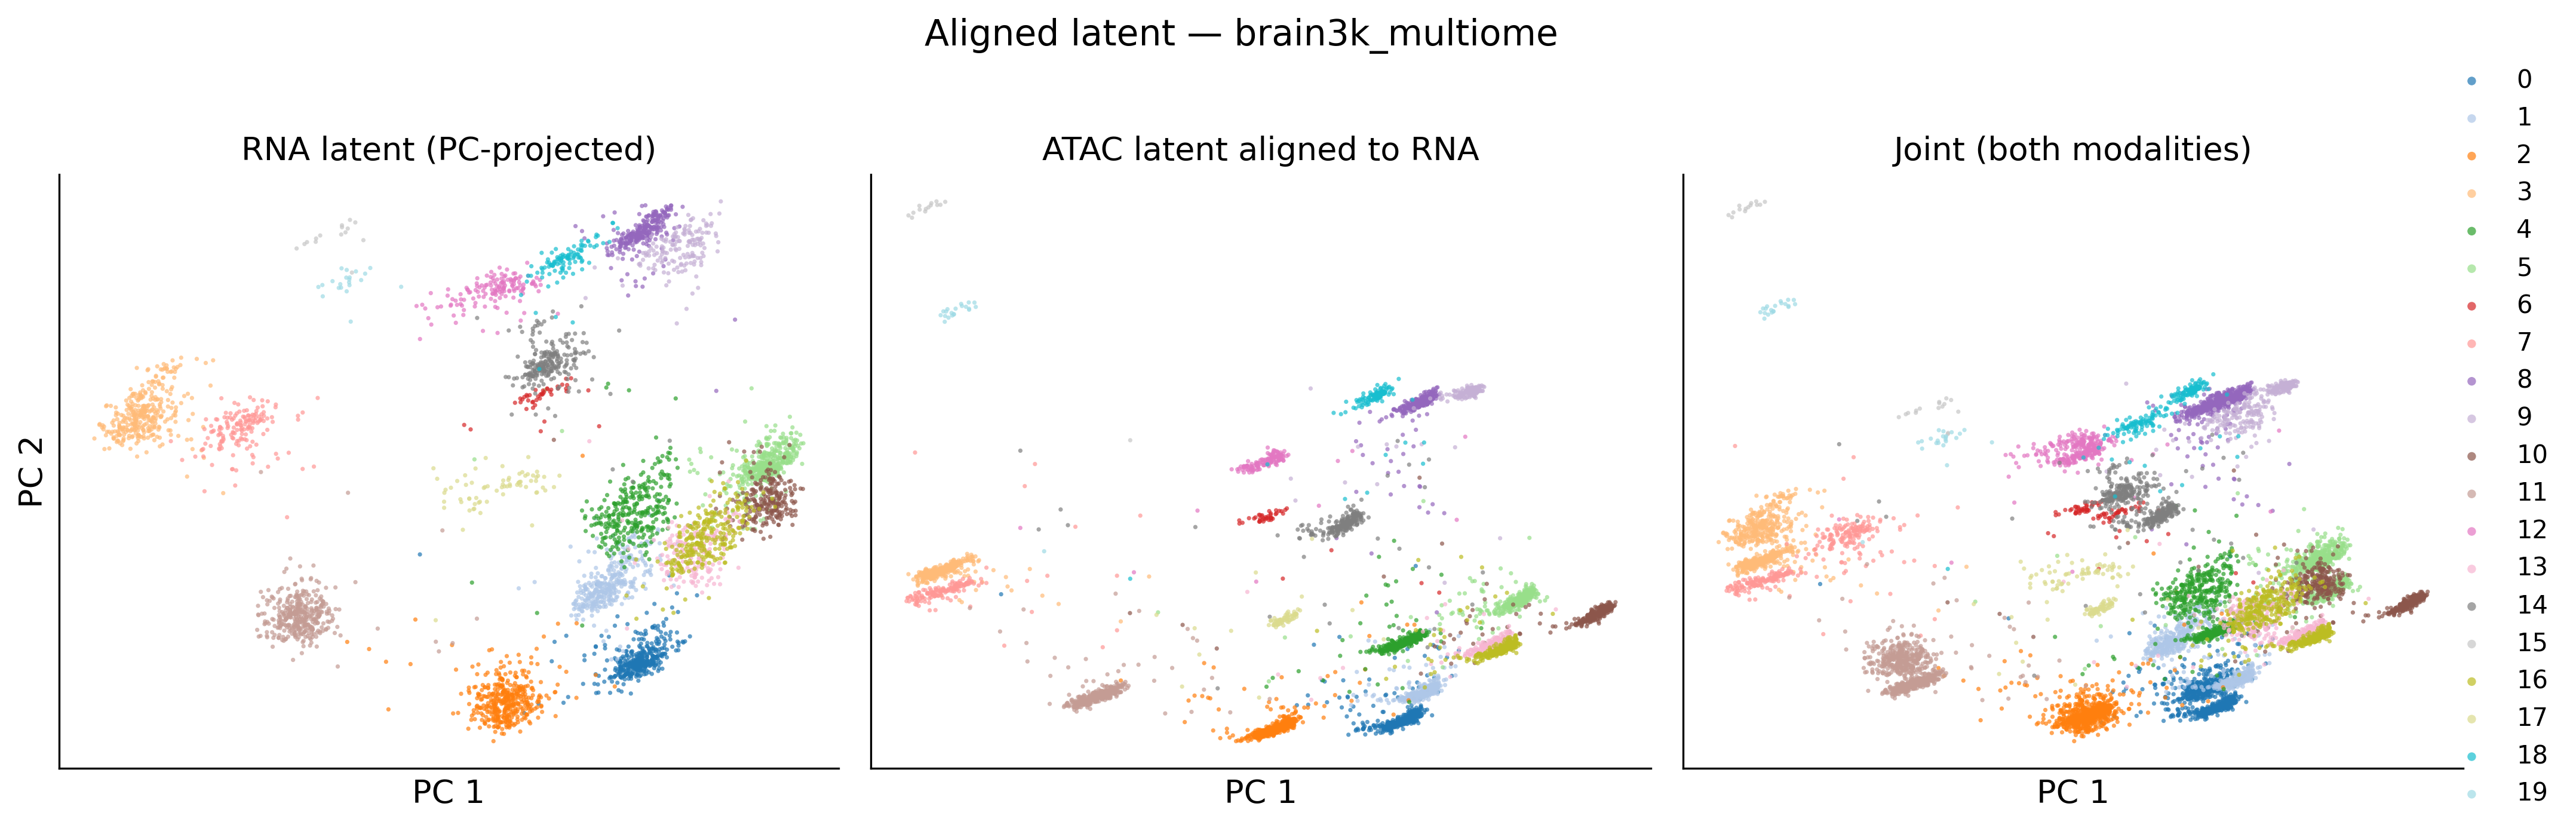
\includegraphics[width=\textwidth]{fig1_aligned_latent_brain3k_multiome.png}
  \caption{\textbf{Supplementary Fig.~S1a: Aligned latent --- neural data (Brain 5k).} Neural progenitor, neuronal, and glial cell-type topology is preserved. Entropy concentrates at transitional states (radial glia$\to$neuron boundaries) and rare clusters.}
\end{figure}

\begin{figure}[h]
  \centering
  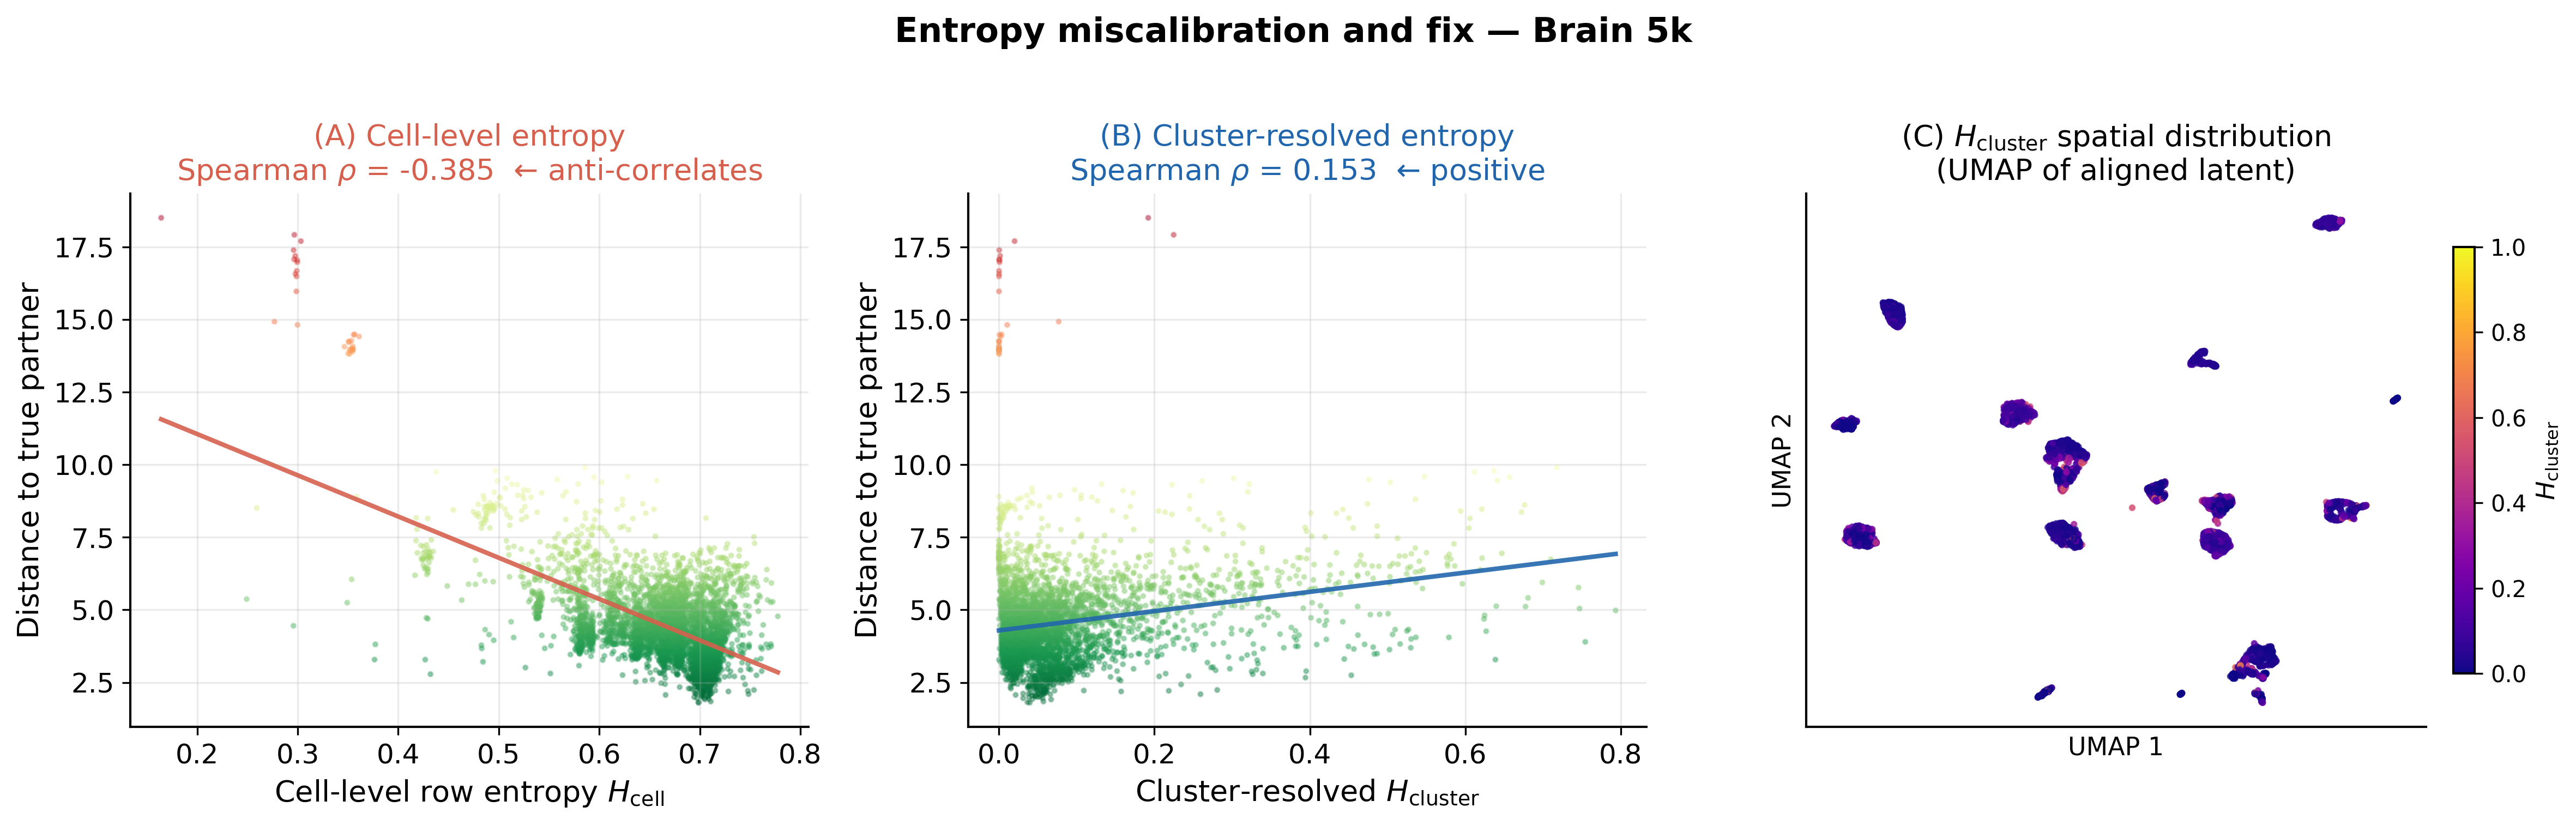
\includegraphics[width=\textwidth]{fig2_entropy_comparison_brain3k_multiome.png}
  \caption{\textbf{Supplementary Fig.~S1b: Entropy miscalibration --- neural data.} Row entropy has the wrong sign ($\rho\approx -0.36$); cluster-resolved entropy is correctly ordered.}
\end{figure}

\textbf{Fig.~S2} ($\beta$ sensitivity): $\beta = 0.001$ is the recommended default. Uncertainty AUROC is roughly insensitive to $\beta$, so the uncertainty signal is robust to this choice.

\begin{figure}[h]
  \centering
  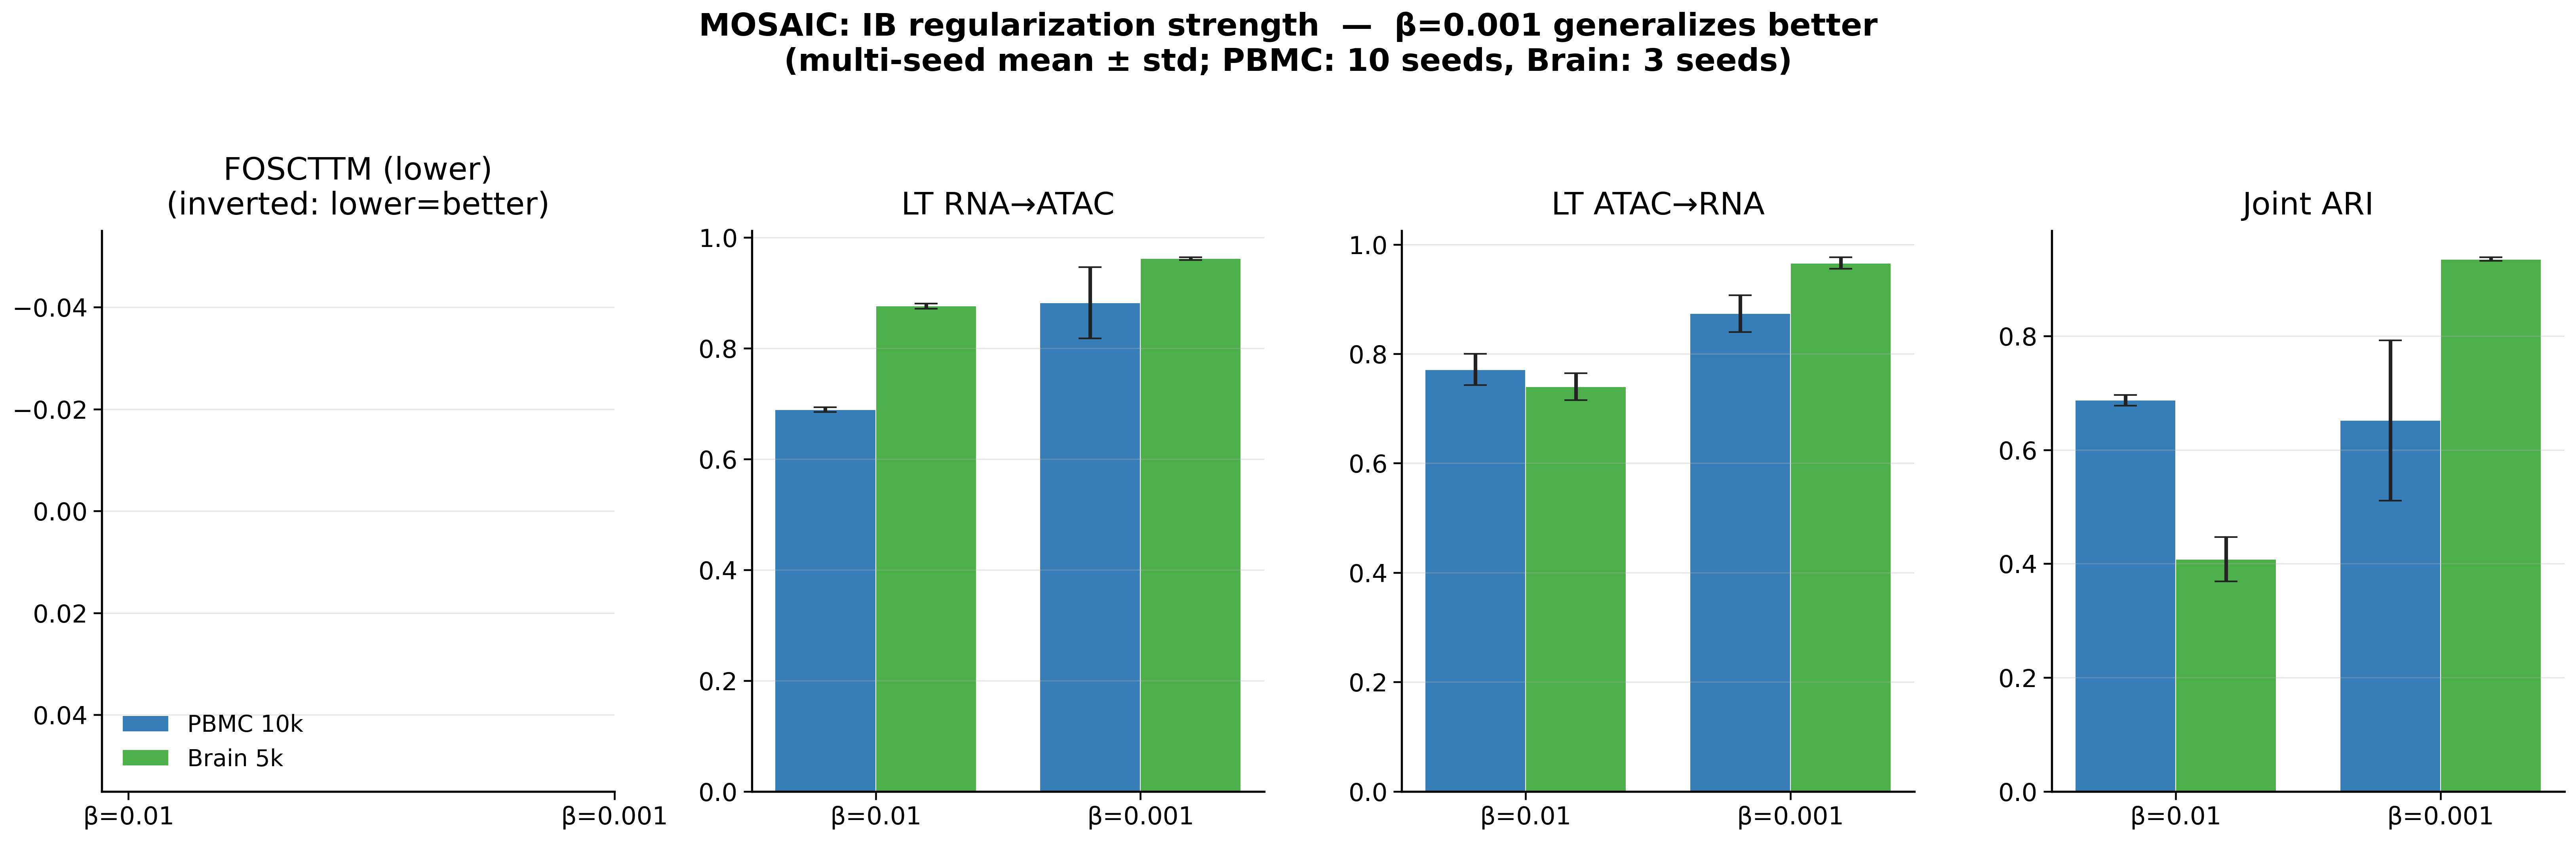
\includegraphics[width=\textwidth]{fig5_beta_tradeoff.png}
  \caption{\textbf{Supplementary Fig.~S2: $\beta$ sensitivity on immune and neural data.} Alignment metrics improve with smaller $\beta$; uncertainty AUROC is stable across the range tested.}
\end{figure}

\textbf{Fig.~S3} (cross-tissue negative control): Full entropy distribution for PBMC$\times$Brain cross-tissue alignment.

\begin{figure}[h]
  \centering
  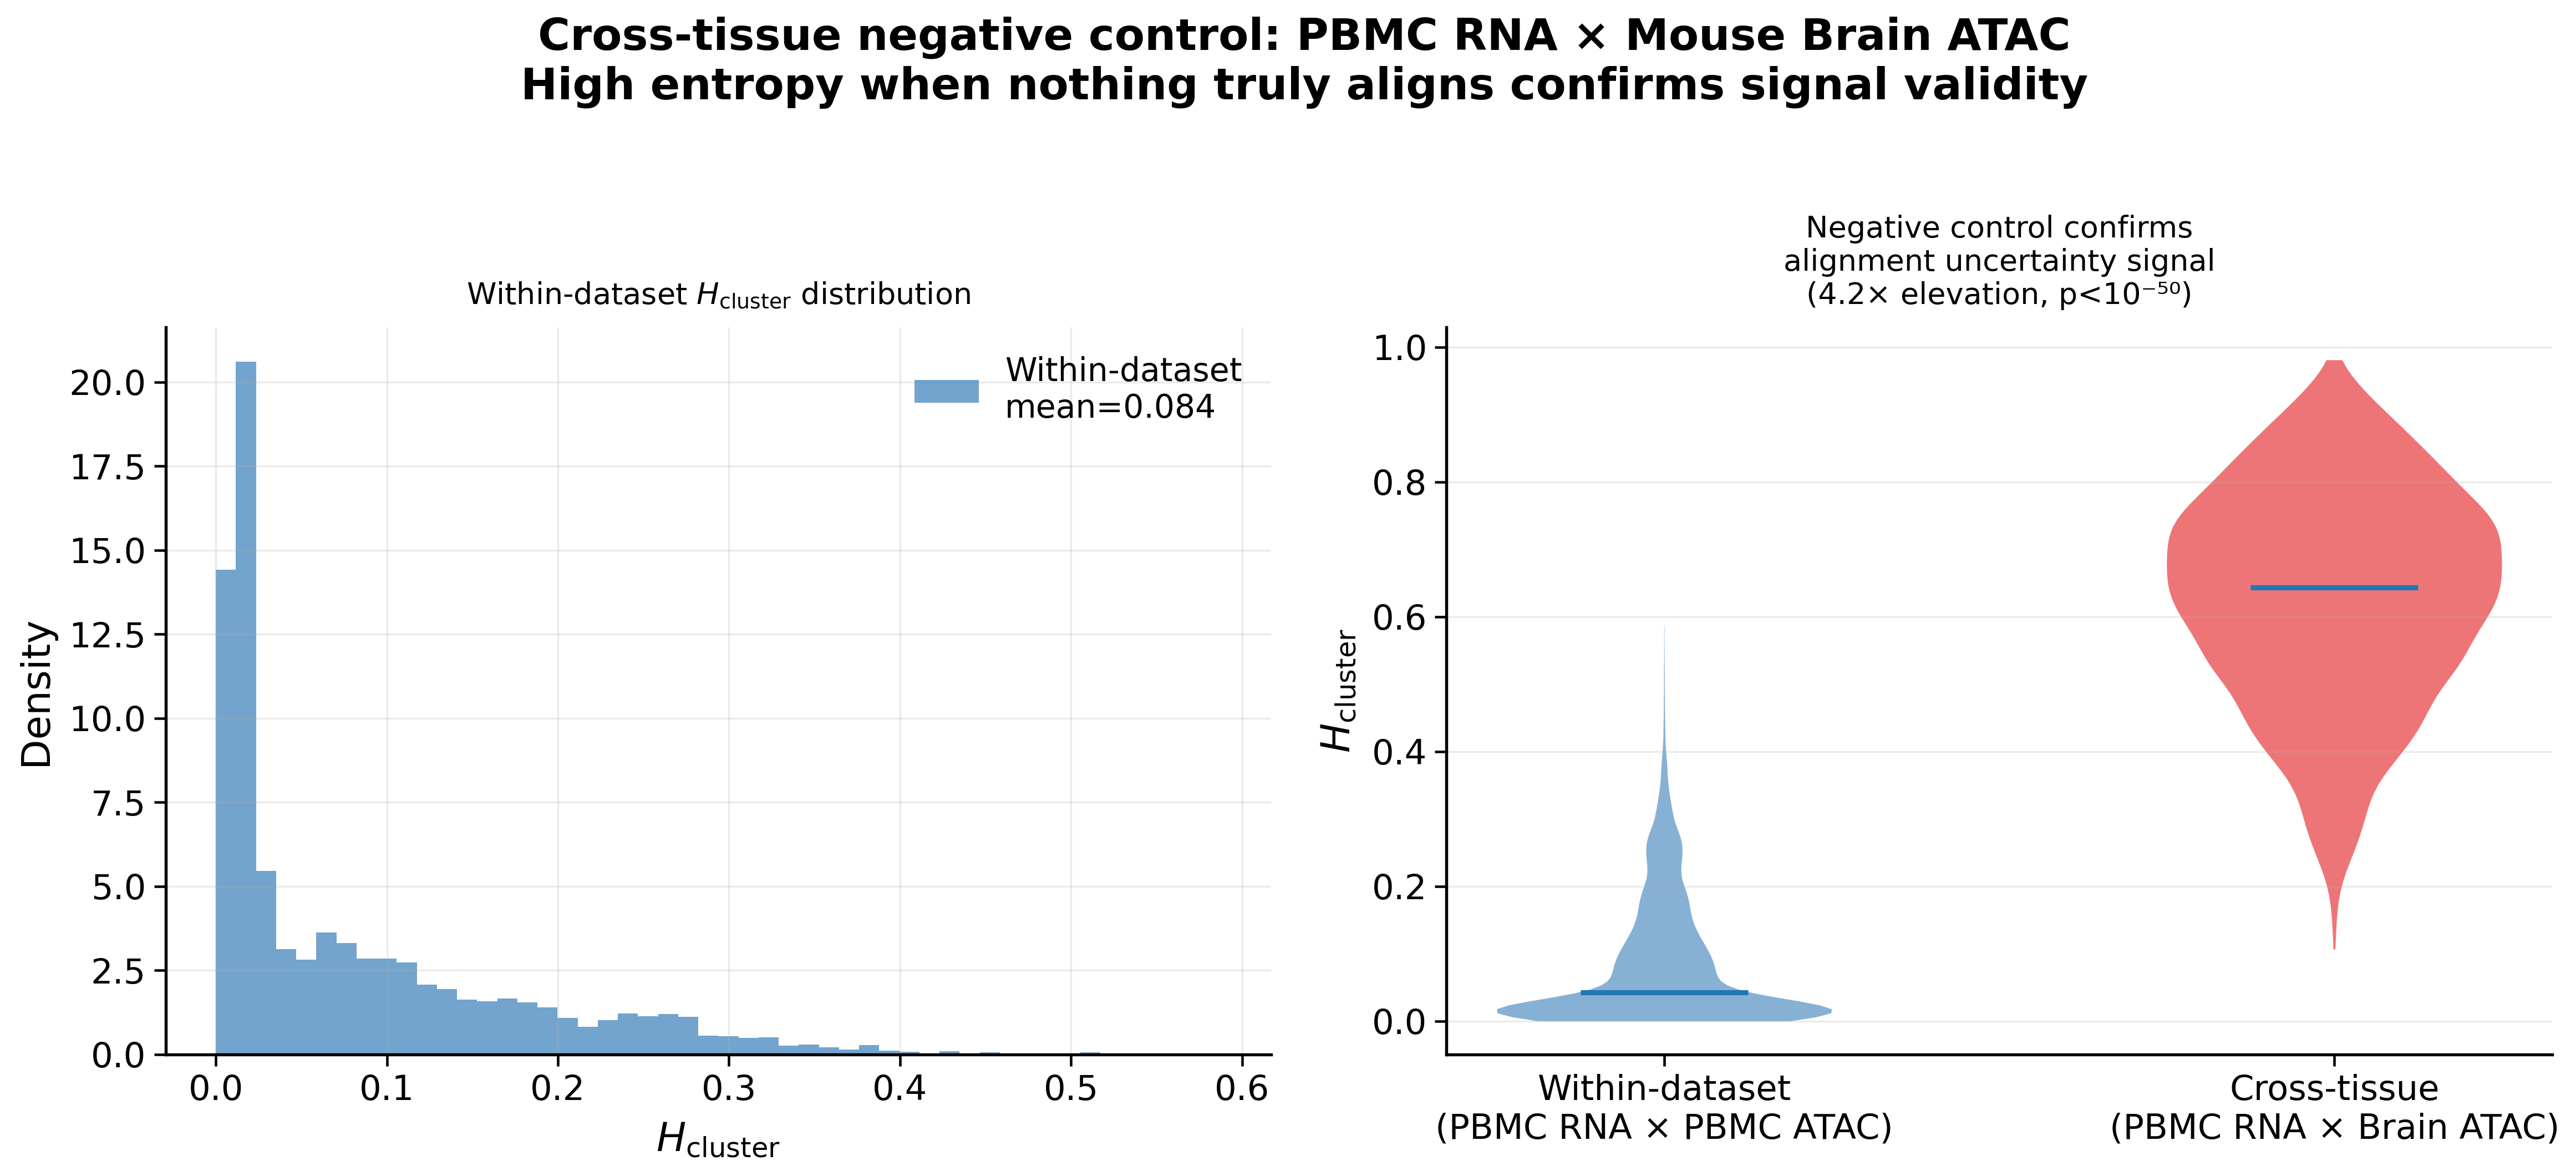
\includegraphics[width=\textwidth]{fig6_cross_tissue_negative_control.png}
  \caption{\textbf{Supplementary Fig.~S3: Cross-tissue negative control.} PBMC RNA aligned against mouse-brain ATAC (zero shared cell types). Mean cluster entropy is $4.2\times$ higher than within-dataset controls.}
\end{figure}

\textbf{Fig.~S4} (calibration and cross-seed stability): Calibration curves and cross-seed reliability analysis.

\begin{figure}[h]
  \centering
  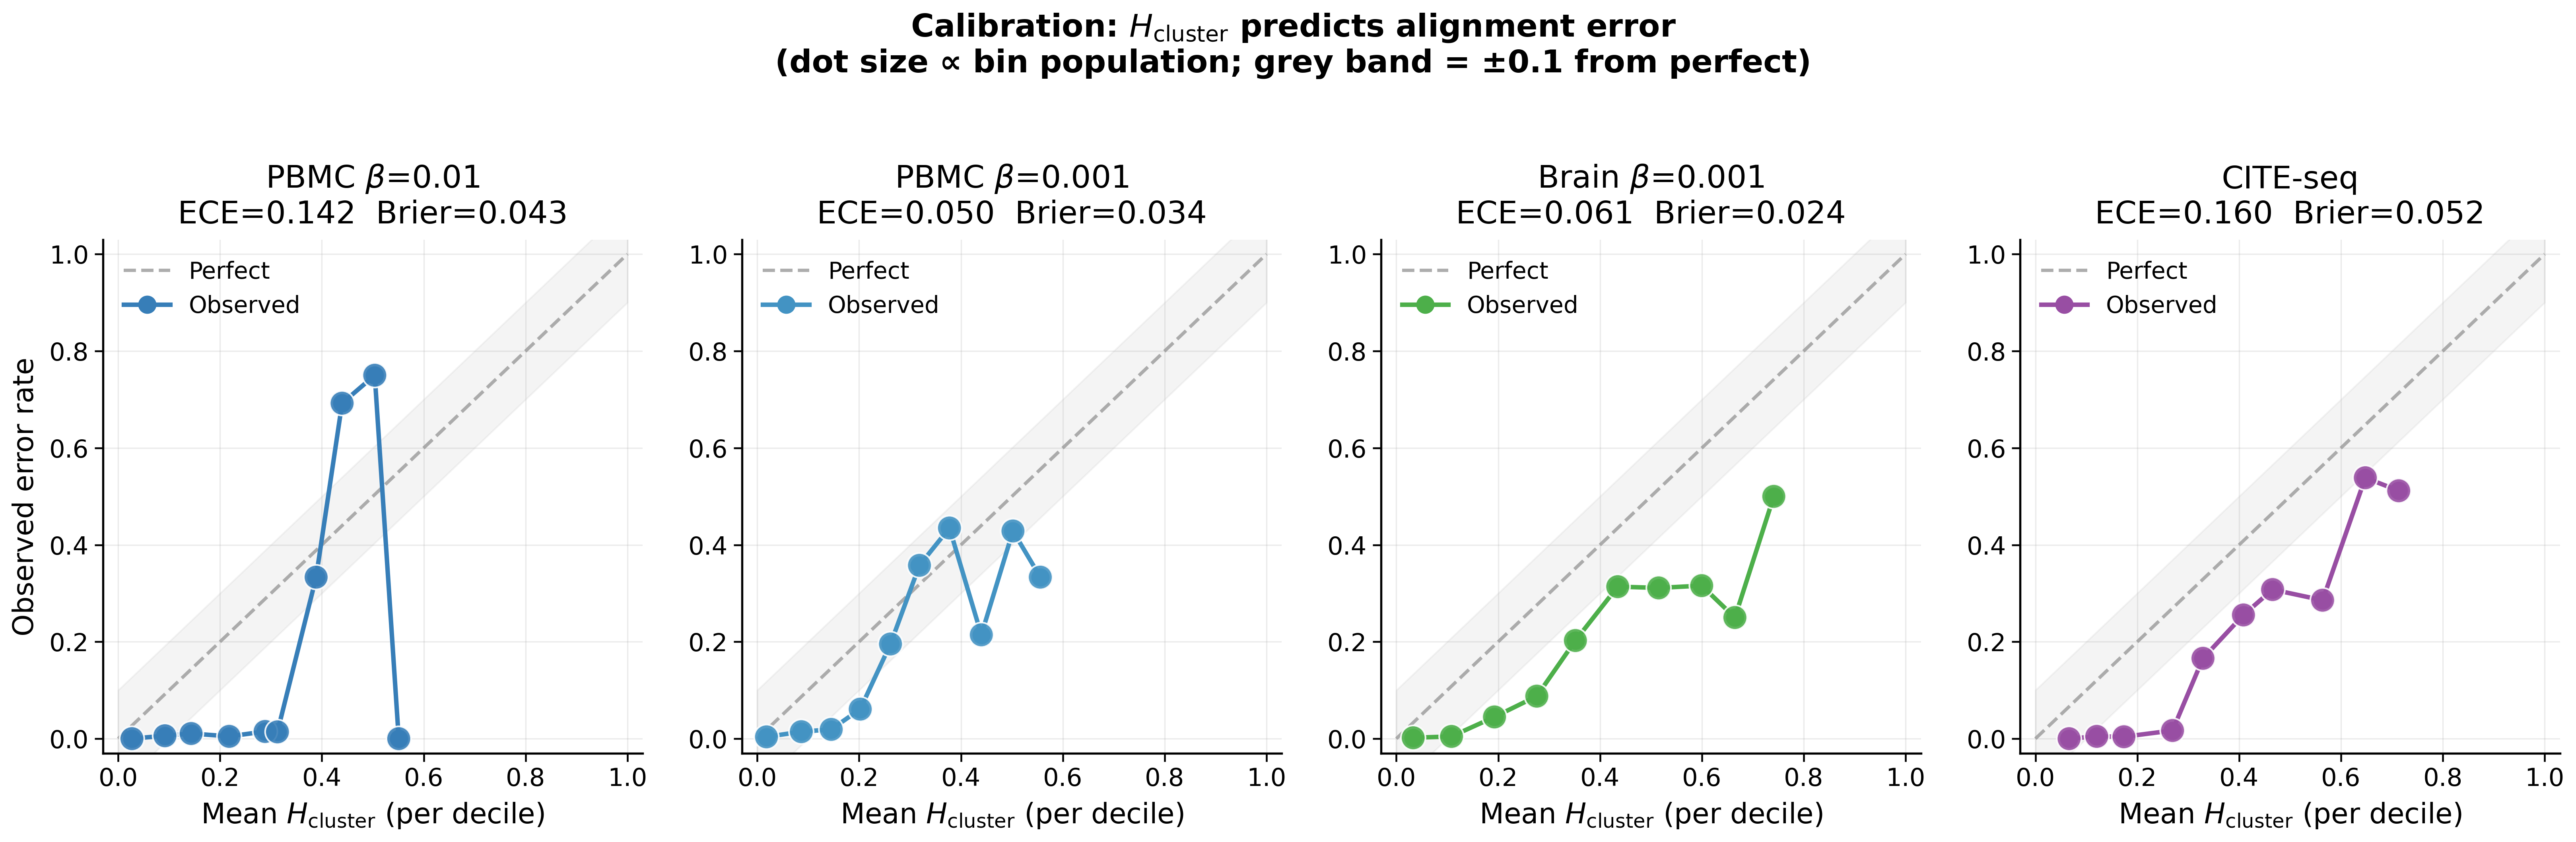
\includegraphics[width=\textwidth]{fig7_calibration_curves.png}
  \caption{\textbf{Supplementary Fig.~S4: Calibration curves.} Mean $\Hcluster$ per decile vs.\ observed error rate: monotonically increasing on all datasets (expected calibration error 0.05--0.16). Multi-seed Brier scores 0.024--0.052.}
\end{figure}

\textbf{Fig.~S5} (disease simulation): Per-disease-scenario AUROC for five immune and five neurological disease simulations.

\begin{figure}[h]
  \centering
  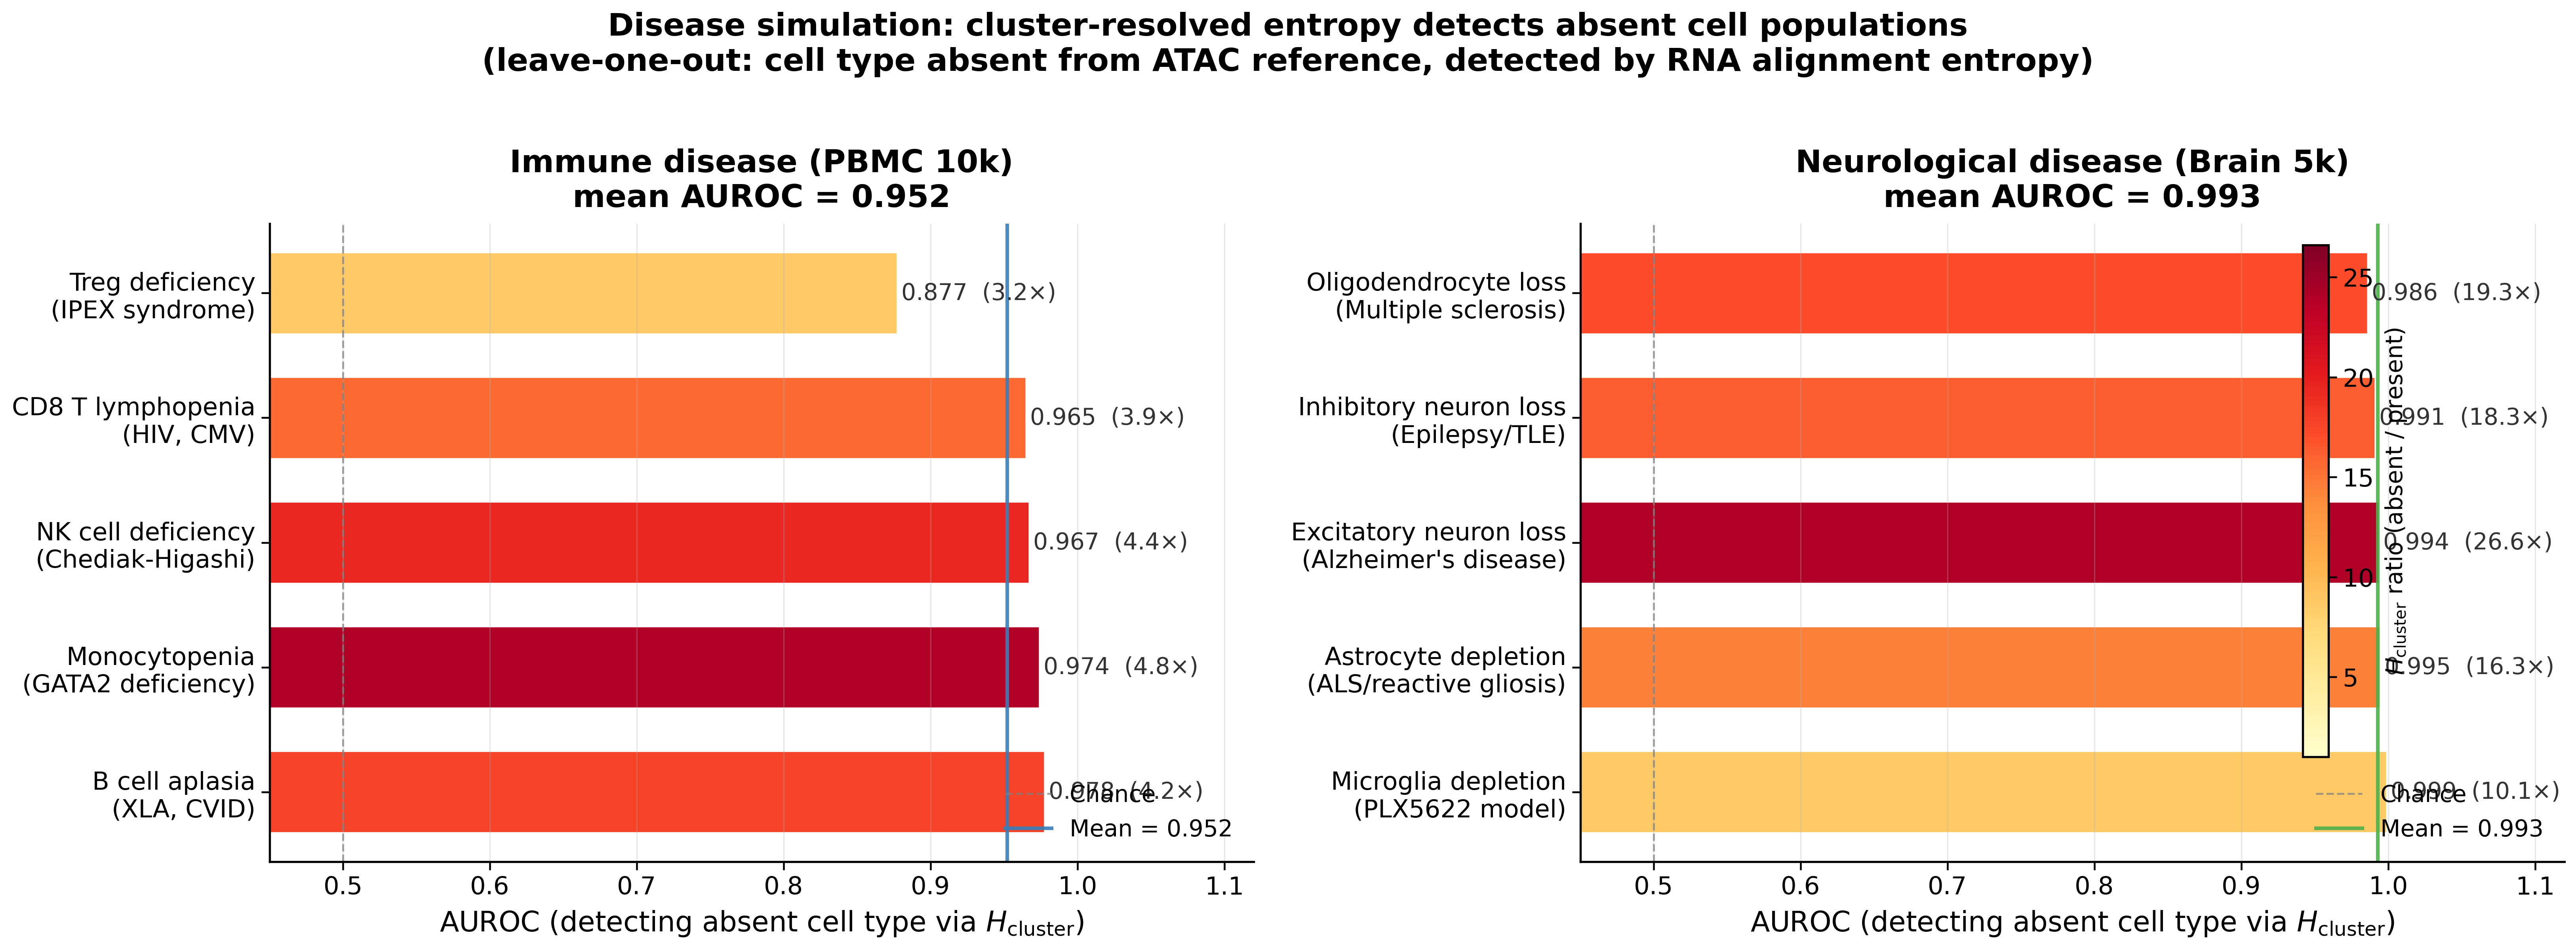
\includegraphics[width=\textwidth]{fig8_disease_simulation.png}
  \caption{\textbf{Supplementary Fig.~S5: Disease simulation.} Mean AUROC 0.952 (immune diseases) and 0.993 (neurological diseases). Bar color encodes entropy ratio (absent/present $\Hcluster$).}
\end{figure}

\textbf{Fig.~S6} (protein marker uncertainty): Surface protein expression in high- vs.\ low-uncertainty cells (CITE-seq).

\begin{figure}[h]
  \centering
  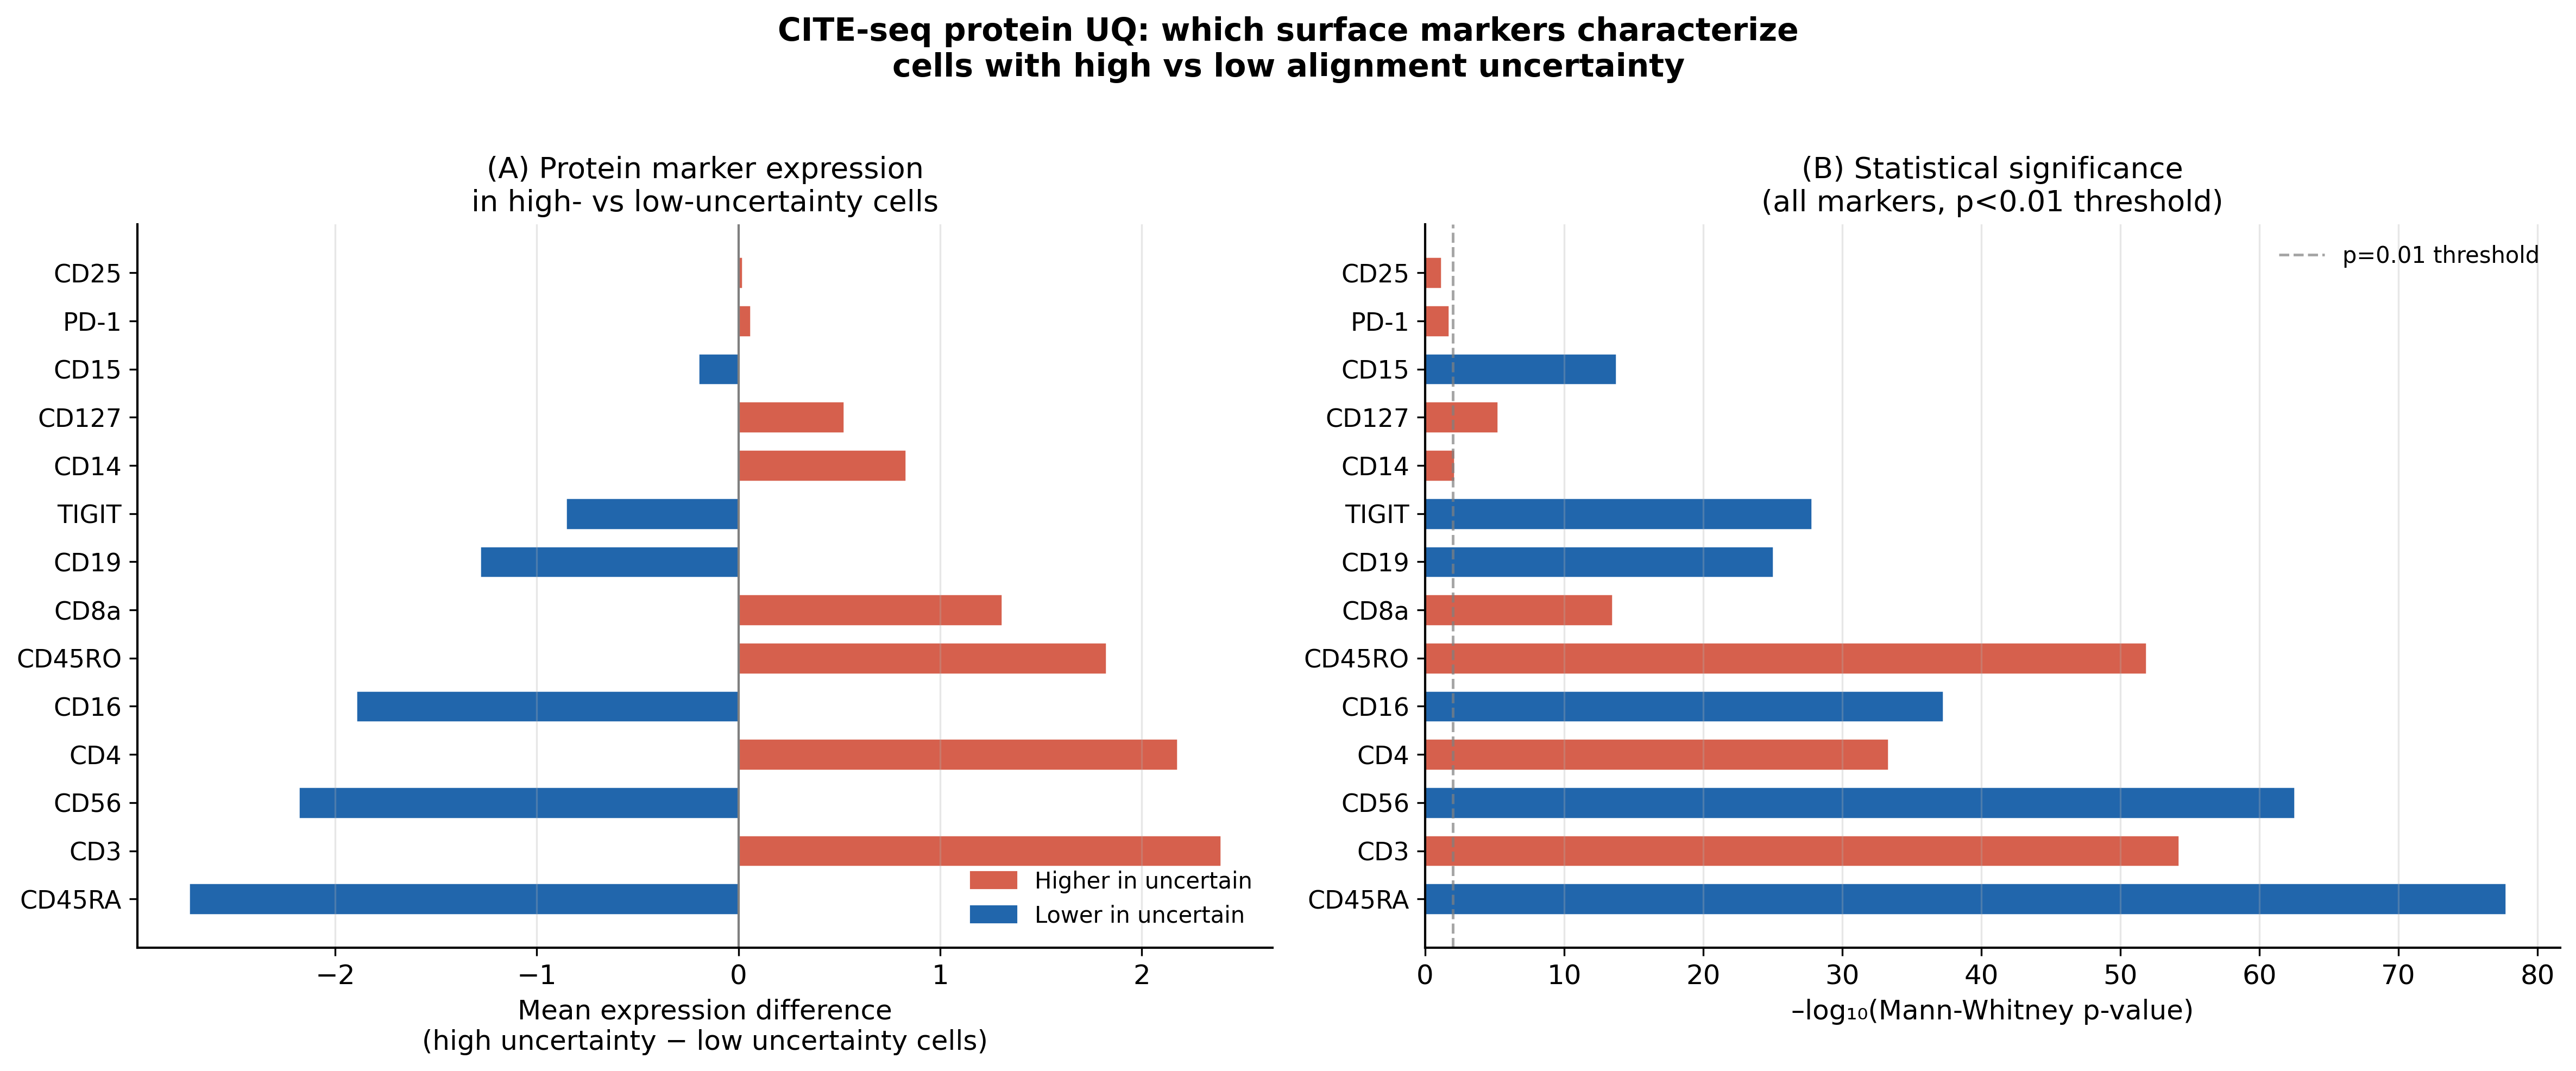
\includegraphics[width=\textwidth]{fig9_protein_uq.png}
  \caption{\textbf{Supplementary Fig.~S6: Protein marker uncertainty (CITE-seq).} T-cell markers enriched in uncertain cells; lineage-committed NK/naive-T markers depleted. All markers significant at $p < 10^{-13}$.}
\end{figure}

\textbf{Fig.~S7} (checkpoint immunotherapy): Alignment uncertainty in exhausted T cells.

\begin{figure}[h]
  \centering
  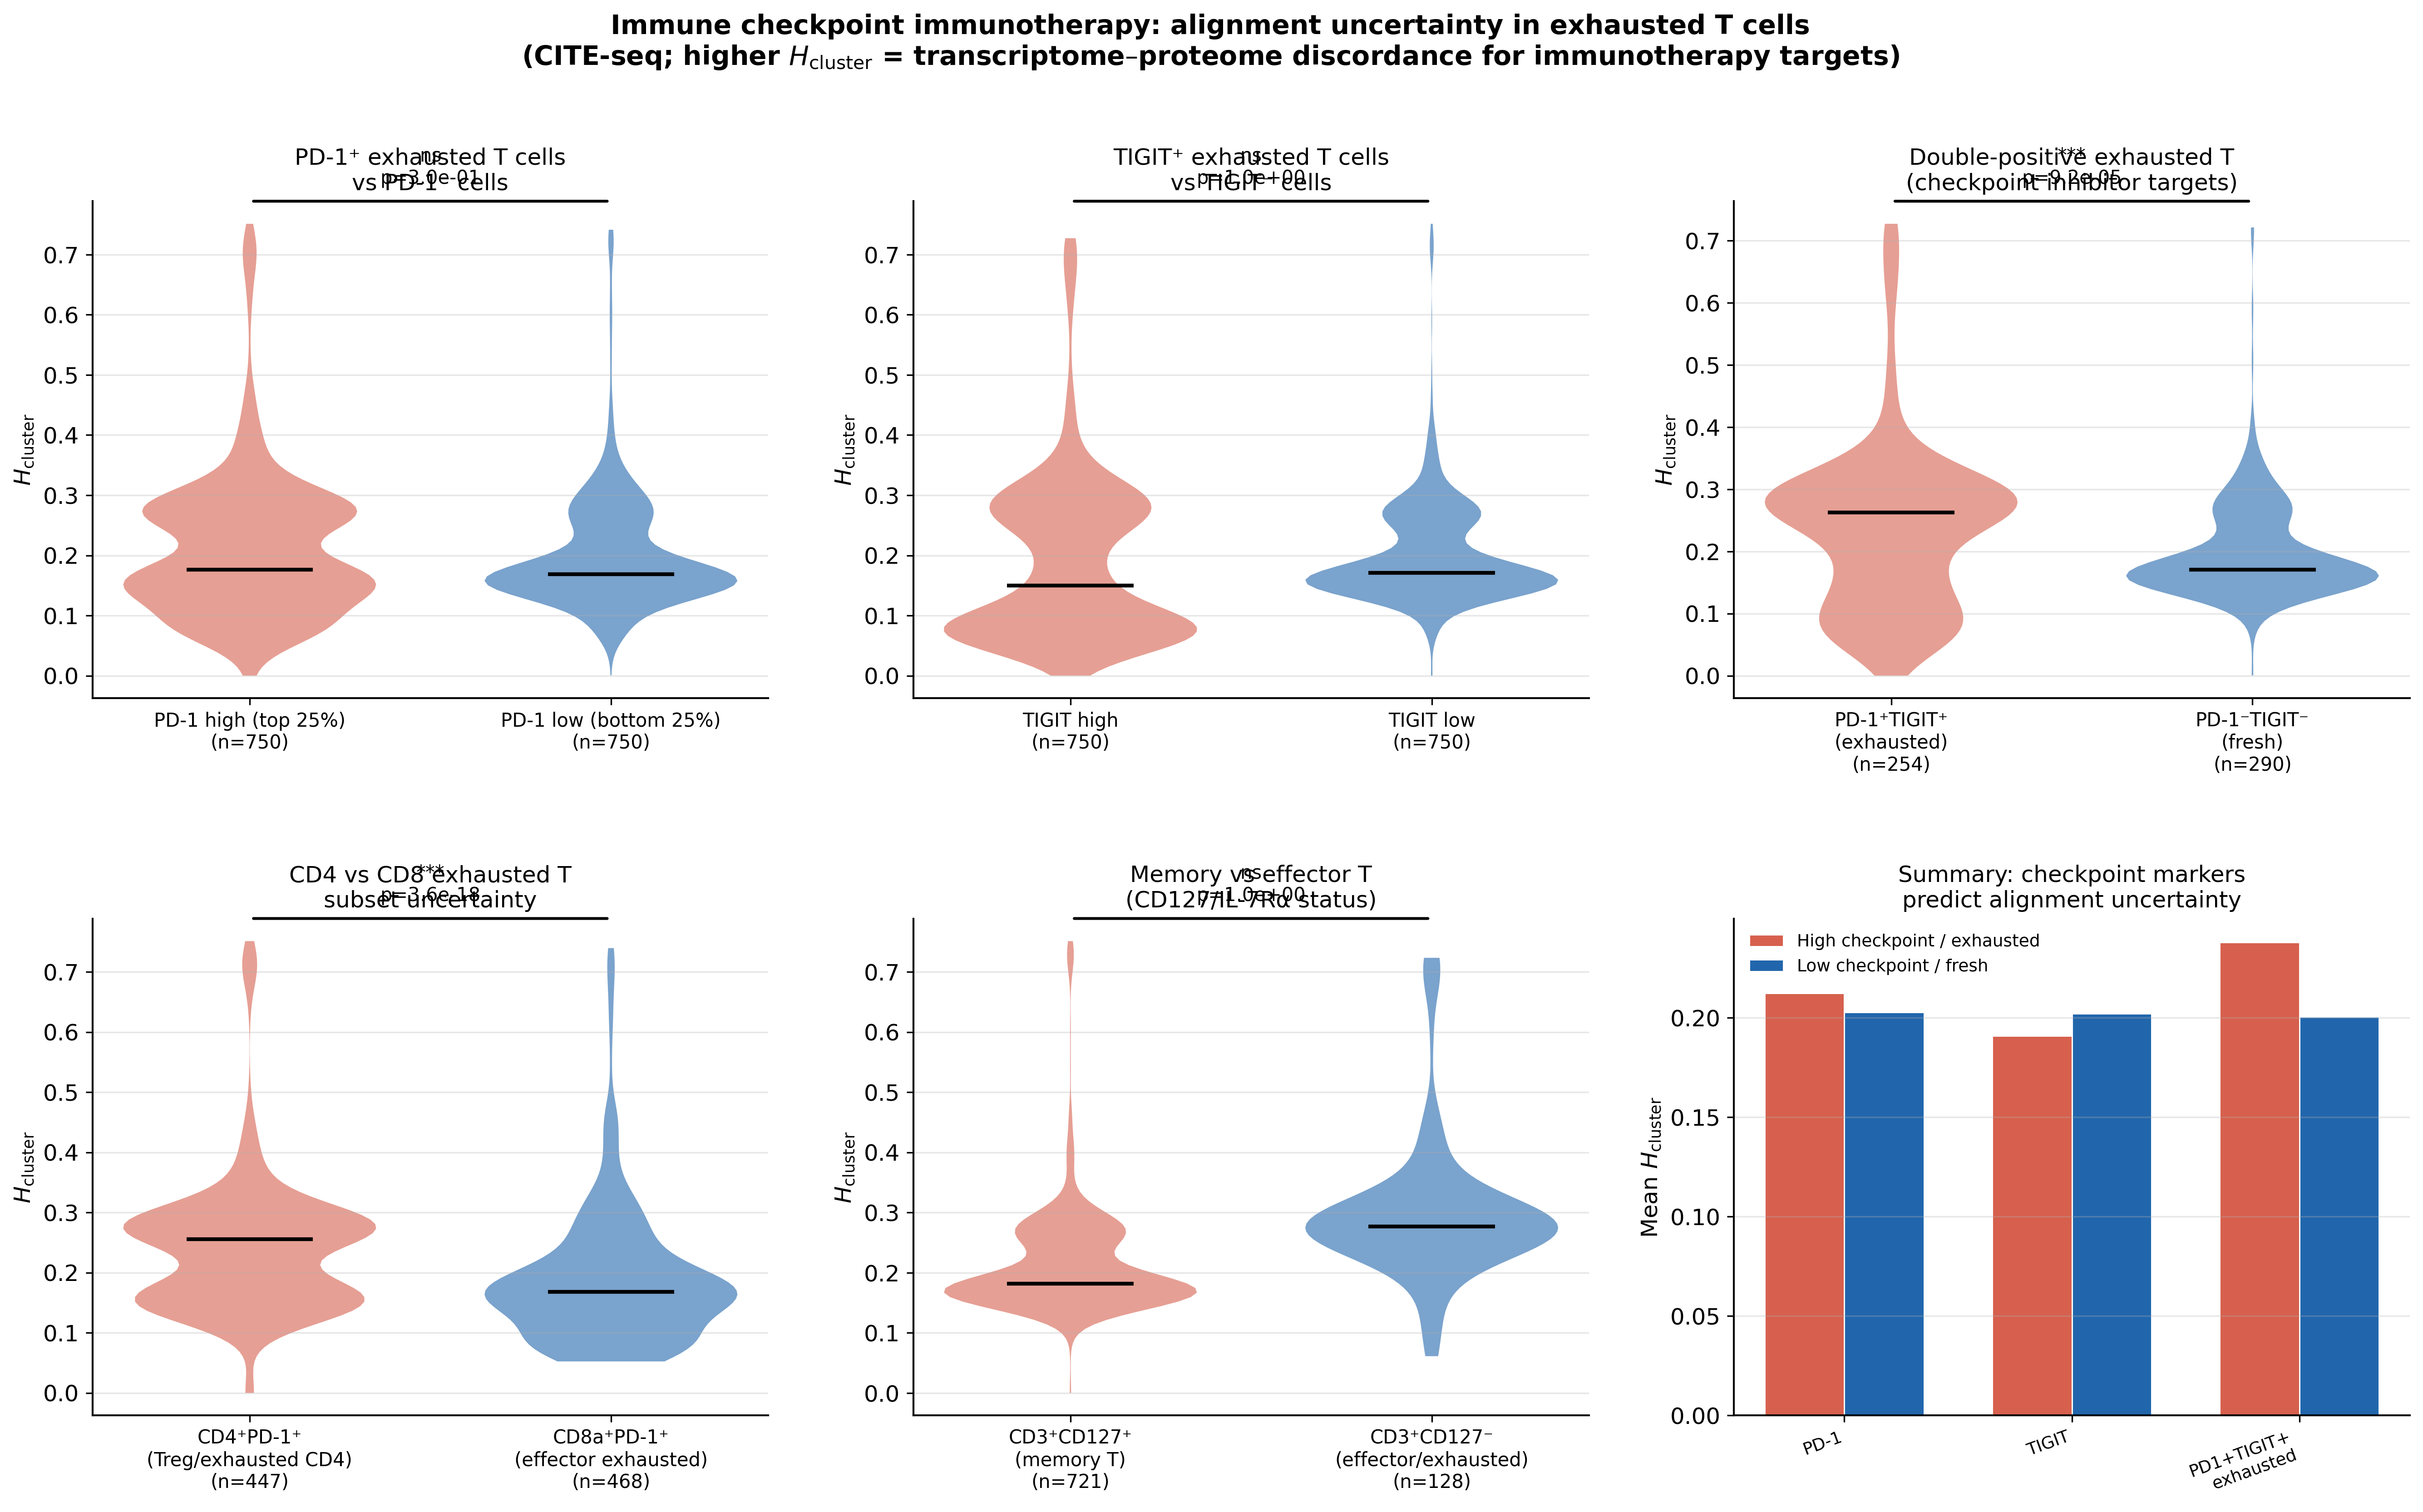
\includegraphics[width=\textwidth]{fig10_checkpoint_immunotherapy.png}
  \caption{\textbf{Supplementary Fig.~S7: Checkpoint immunotherapy entropy.} Exhausted T cells (PD-1$^+$, TIGIT$^+$, double-positive) show higher alignment uncertainty; CD4$^+$PD-1$^+$ cells more uncertain than CD8a$^+$PD-1$^+$.}
\end{figure}

\subsection*{C. Multi-seed aggregate results}

\begin{table}[h]
\centering
\caption{\textbf{Supplementary Table~S1}: Multi-seed means $\pm$ std (3 seeds for neural and proteomic data; 10 seeds for immune $\beta=0.001$).}
\label{tab:multiseed}
\begin{tabular}{llrrrr}
\toprule
\textbf{Dataset} & $\beta$ & FOSCTTM & LT A$\to$B & LT B$\to$A & ARI \\
\midrule
PBMC 10k & 0.01  & $0.188 \pm 0.006$ & $0.689 \pm 0.005$ & $0.771 \pm 0.029$ & $\mathbf{0.687 \pm 0.009}$ \\
PBMC 10k & \textbf{0.001} & $\mathbf{0.118 \pm 0.008}$ & $\mathbf{0.913 \pm 0.074}$ & $\mathbf{0.909 \pm 0.035}$ & $0.724 \pm 0.103$ \\
Brain 5k & 0.01  & $0.129 \pm 0.004$ & $0.877 \pm 0.005$ & $0.740 \pm 0.025$ & $0.408 \pm 0.039$ \\
Brain 5k & \textbf{0.001} & $\mathbf{0.049 \pm 0.002}$ & $\mathbf{0.962 \pm 0.002}$ & $\mathbf{0.966 \pm 0.010}$ & $\mathbf{0.935 \pm 0.003}$ \\
\bottomrule
\end{tabular}
\end{table}

\subsection*{D. Compute and reproducibility}

End-to-end wall time on a single NVIDIA RTX 3080 (16~GB): $\sim$120~s per immune run, $\sim$50~s per neural run, $\sim$95~s per proteomic run. Memory peak $\sim$8~GB at $5000\times5000$ cost matrix in float64. All random seeds are set deterministically (NumPy, PyTorch, cuDNN); multi-seed results are aggregated over seeds 0--9 (immune $\beta=0.001$) and seeds 0--2 (all other configurations). An anonymized release of the full codebase, configurations, and experiment JSON files is available at the repository linked from the title page.

\end{document}
